\chapter{Sobel Sequences -- Background and Empirical Data}\labch{SS}
In this chapter, we examine Sobel sequences as well as reverse Sobel sequences, and attempt to identify which factors decide the (in-)felicity of the latter. To this end, we first revisit what (reverse) Sobel sequences, the variably-strict conditional semantics, and (semi-)dynamic strict semantics are in \refsec{sobelbg}. Then, in \refsec{sobelklecha}, we take a closer look at both the empirical findings and the proposed model for reverse Sobel sequence (in-)felicity of \textcite{Klecha2014,Klecha2015}. In \refsec{karenlewis}, we examine another recent proposal for reverse Sobel sequences, which is based upon a dynamic world ordering system \parencite{Lewis2016} and the assumption that world dissimilarity correlates with reverse Sobel sequence felicity \parencite{Lewis2018}. We strengthen her model in \refsec{lewis-klecha} and then experimentally test the claims made about reverse Sobel sequences in \refsec{experiment}. Finally, in \refsec{introspection}, we use the insights gleaned from the previous sections and untangle the factors that determine reverse Sobel sequence (in-)felicity.

\section{Background}\labsec{sobelbg}
Sobel sequences \parencite{Lewis1973,Sobel1970} are sequences of (typically counterfactual) conditionals where the second conditional's antecedent conjoins an additional proposition to the previous conditional's antecedent and results in the negation of the previous conditional's consequent. The most commonly cited example for Sobel sequences is \refex{SS-nuclear}, as originally provided by \textcite[p. 10]{Lewis1973}.
\ex\phantomsection\labex{SS-nuclear}If the USA threw its weapons into the sea tomorrow, there would be war;\linebreak but if the USA and the other nuclear powers all threw their weapons into the sea tomorrow, there would be peace.\hfill\parencite[p. 10]{Lewis1973}
\xe
Although this example was originally put forth as a sequence of counterfactual conditionals, and most of the initial (and contemporary) research on Sobel sequences focused almost entirely on counterfactual Sobel sequences, \refex{SS-nuclear} is actually a sequence of future-less-vivid conditionals \parencite{Iatridou2000}. This is in line with subsequent research which showed that Sobel sequences are not restricted to counterfactuality. In fact, any type of sequence of conditionals---be they indicative \parencite{Williams2008}, predictive \parencite{Moss2012,Willer2013}, future-less-vivid, or counterfactual---may be a Sobel sequence, as pointed out by \textcite{Williams2008}, \textcite{Willer2017}, and \textcite{Klecha2014,Klecha2015}, amongst others. We would therefore define Sobel sequences as follows:
\ex\phantomsection\labdef{SS}\extitle{Sobel Sequence}A Sobel sequence is any sequence of conditionals that adheres to the pattern of \enquote{If $\phi$, $\chi$; [but] if $(\phi\land\psi)$, $\neg\chi$}, where $\phi\neq\psi$.%

\xe
Originally, Sobel sequences were used to argue in favour of the non-monotonicity of counterfactual conditionals' domains of quantification: If counterfactual conditionals were indeed downward monotone, further restricting the antecedent with another proposition would not change the overall truth value of the conditional. In other words, a more restrictive antecedent cannot yield a different consequent than its less restrictive counterpart. If they were upward monotone, on the other hand, the initial conditional would be evaluated as false, as the truth value derived for the more domain-restricted second conditional would also be enforced for the less domain-restricted first conditional. As shown by the Sobel sequence in \refex{SS-nuclear}, it is clear that neither option appears to be the case.

This was an important observation, as the predominant analysis at that time---known as the strict conditional analysis---predicted counterfactual conditionals to be downward monotone with regard to their quantificational domain.  It assumed that (subjunctive) conditionals were to be analysed as a necessity modal quantifying over the material implication, as originally proposed by \textcite[p. 33]{Peirce1896}, defended and elaborated upon by \textcite{Lewis1912,Lewis1914,Lewis1918}, and formalised below in its modern standard form, using \citepos{Kripke1963} modal logic semantics:
\ex\phantomsection\labex{strict}$\intension{If $\phi$, $\psi$.}=\textiff\square(\phi\rightarrow\psi)$
\xe
In other words, it was assumed that the consequent must be considered true for all possible worlds that satisfy the specifications of the antecedent. This assumption would have rendered the antecedent of conditionals downward monotonic. For Sobel sequences, that would have meant that the $\phi$-conditional also quantifies over the $\phi\land\psi$-worlds of the subsequent $\phi\land\psi$-conditional, thereby yielding contradictory claims concerning whether $\chi$ is true in these aforementioned worlds or not.
\subsection{Variably-Strict Semantics}
A model of conditionals with more accurate predictions concerning Sobel sequences was then formulated by \textcite{Stalnaker1968} and \textcite{Lewis1973}, who introduced the notion that a conditional does not simply quantify over all possible worlds, but merely over a subset of these worlds---namely those possible worlds that fulfil the requirements of the antecedent and that can be considered the least different to the world the conditional was uttered in (referred to as the evaluation world, which typically though not necessarily coincides with the actual world $w_0$). To this end, they have introduced the notions of worlds similarity and world closeness, which have been treated near-synonymously by most semanticists until relatively recently: World closeness determines the ranking of each possible world in relation to some evaluation world by some measure. This measure has traditionally been world similarity. World similarity measures how similar a possible world should be considered to the evaluation world, and was nigh-simultaneously developed by \textcite{Stalnaker1968},\linebreak \textcite{Stalnaker1970}, \textcite{Sprigge1970}, \textcite{Lewis1973}, and \textcite{Nute1975}, but first formulated as a notion by \textcite[p. 107]{Todd1964}:
\begin{displayquote}
When we allow for the possibility of the antecedent’s being true in the case of a counterfactual, we are hypothetically substituting a different world for the actual one. It has to be supposed that this hypothetical world is as much like the actual one as possible so that we will have grounds for saying that the consequent would be realised in such a world.
\end{displayquote}
To this end, \textcite{Lewis1973} counts any additional deviation from the evaluation world as an increase in dissimilarity.\footnote{The view that similarity decreases with each and every deviation from the evaluation world leads to a number of problems down the line. A more sensible approach concerning how world similarity is to be measured is introduced in \refsec{css-bennett-explanation} and reflects the work of \textcite{Bennett2003} and \textcite{Arregui2009}.} This similarity ordering is traditionally visually represented by concentric layers, where each layer further out represents an additional decrease in similarity to the evaluation world found at the centre, as seen in \reffig{similarity-ordering}.
\begin{figure}[!htb]
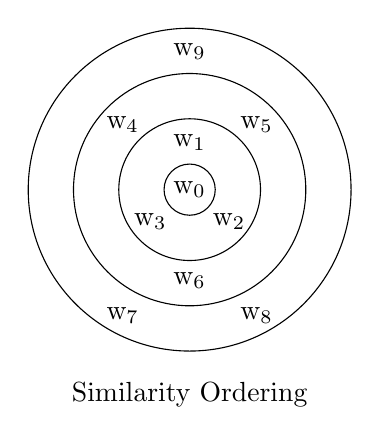
\begin{tikzpicture}
	\coordinate (O) at (0,0);

	\draw[fill=white] (O) circle (2.05);
	\draw[fill=white] (O) circle (1.475);
	\draw[fill=white] (O) circle (0.9);
	\draw[fill=white] (O) circle (0.325)node {w$_0$};

	\node at (0,0.6) {w$_1$};
	\node at (0.5,-0.4) {w$_2$};
	\node at (-0.5,-0.4) {w$_3$};
	
	\node at (-0.85,0.825) {w$_4$};
	\node at (0.85,0.825) {w$_5$};
	\node at (0,-1.15) {w$_6$};
	
	\node at (-0.85,-1.6) {w$_7$};
	\node at (0.85,-1.6) {w$_8$};
	\node at (0,1.75) {w$_9$};
	
	\node at (0,-2.6) {Similarity Ordering};
\end{tikzpicture}
\caption{Similarity ordering with respect to the evaluation world $w_0$, where the worlds $w_{1\leqslant n\leqslant3}$ are equally similar to $w_0$, but more similar to $w_0$ than $w_{4\leqslant n\leqslant9}$, and where $w_{4\leqslant n\leqslant6}$ are still more similar to $w_0$ than $w_{7\leqslant n\leqslant9}$.}
\labfig{similarity-ordering}
\end{figure}

We therefore define the variably-strict analysis's conditional semantics as follows:
\ex\phantomsection\labdef{variablystrict}For all contexts $c$, \enquote{If $\phi$, $\psi$} is true at $w$ in $c$ iff all the closest $\phi$-worlds to $w$ are $\psi$-worlds, where closeness is determined by similarity.%

\xe
This effectively renders counterfactual conditionals non-monotonic in their domain of quantification. Applied to Sobel sequences, this would mean that the $\phi$-conditional no longer quantifies over the worlds of the $\phi\land\psi$-conditional. Instead, the two conditionals quantify over two entirely disjoint sets of worlds, as shown in \reffig{stalnakerlewis-SS}. As such, no contradictory claim is made, rendering Sobel sequences perfectly felicitous.
\begin{figure}[!htb]
    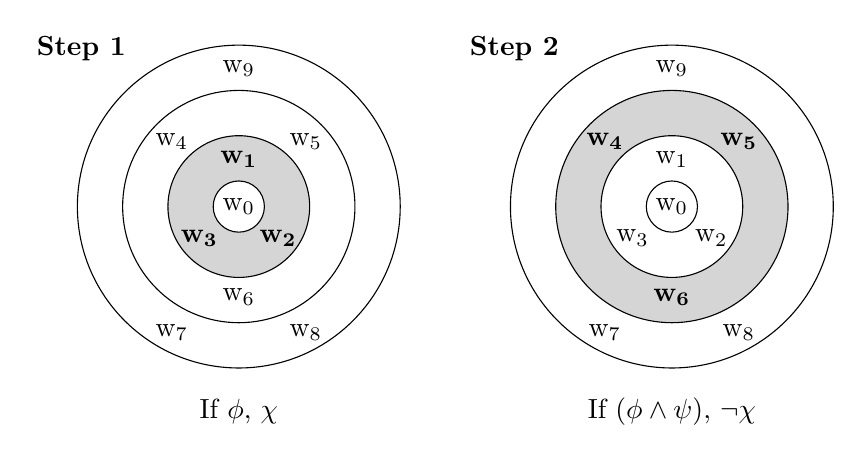
\begin{tikzpicture}
	\coordinate (O) at (0,0);
    \node at (-2,2) {\textbf{Step 1}};
	\draw[fill=white] (O) circle (2.05);
	\draw[fill=white] (O) circle (1.475);
	\draw[fill=gray!33] (O) circle (0.9);
	\draw[fill=white] (O) circle (0.325)node {w\textsubscript{0}};

	\node at (0,0.6) {\textbf{w\textsubscript{1}}};
	\node at (0.5,-0.4) {\textbf{w\textsubscript{2}}};
	\node at (-0.5,-0.4) {\textbf{w\textsubscript{3}}};
	
	\node at (-0.85,0.825) {w\textsubscript{4}};
	\node at (0.85,0.825) {w\textsubscript{5}};
	\node at (0,-1.15) {w\textsubscript{6}};
	
	\node at (-0.85,-1.6) {w\textsubscript{7}};
	\node at (0.85,-1.6) {w\textsubscript{8}};
	\node at (0,1.75) {w\textsubscript{9}};
	
	\node at (0,-2.6) {If $\phi$, $\chi$};
	
	
	\begin{scope}[xshift=5.5cm]
		\coordinate (O) at (0,0);
        \node at (-2,2) {\textbf{Step 2}};
    \draw[fill=white] (O) circle (2.05);
	\draw[fill=gray!33] (O) circle (1.475);
	\draw[fill=white] (O) circle (0.9);
	\draw[fill=white] (O) circle (0.325)node {w\textsubscript{0}};

	\node at (0,0.6) {w\textsubscript{1}};
	\node at (0.5,-0.4) {w\textsubscript{2}};
	\node at (-0.5,-0.4) {w\textsubscript{3}};
	
	\node at (-0.85,0.825) {\textbf{w\textsubscript{4}}};
	\node at (0.85,0.825) {\textbf{w\textsubscript{5}}};
	\node at (0,-1.15) {\textbf{w\textsubscript{6}}};
	
	\node at (-0.85,-1.6) {w\textsubscript{7}};
	\node at (0.85,-1.6) {w\textsubscript{8}};
	\node at (0,1.75) {w\textsubscript{9}};
	
	\node at (0,-2.6) {If $(\phi\land\psi)$, $\neg\chi$};
	\end{scope}
\end{tikzpicture}
\caption{Domains of quantification for Sobel sequences according to \textcite{Stalnaker1968} and \citepos{Lewis1973} variably-strict conditional analyses. For all $w_n$-worlds: If $n\geqslant1$, then $\phi=1$ is true for $w_n$, and if $n\geqslant 4$, then $\psi=1$ holds true for $w_n$. If $n\geqslant 7$, then some proposition $\omega=1$ such that $\omega\neq\phi$, $\omega\neq\psi$, and $\phi,\psi$ do not precede $\omega$ on some causal chain of events.}
\labfig{stalnakerlewis-SS}
\end{figure}\vspace{-3mm}

Crucially, since the set of the closest $\phi$-worlds and the set of the closest $\phi\land\psi$-worlds are disjoint, the order in which conditionals make claims about them should be of no further relevance. However, this appears to not be the case: Reverse Sobel sequences---defined in \refdef{rSS}---have traditionally been observed to be infelicitous, even though they, as the name would imply, consist of the same conditionals as a Sobel sequence, merely in reverse order. The infelicity of such sequences is typically demonstrated with the counterpart to \refex{SS-nuclear}, as seen in \refex{rSS-nuclear}, that was originally provided by \textcite{Heim1994}.\vspace{-2mm}
\ex\phantomsection\labdef{rSS}\extitle{Reverse Sobel Sequence}A reverse Sobel sequence is any sequence of conditionals that adheres to the pattern of \enquote{If $(\phi\land\psi)$, $\neg\chi$; [but] if $\phi$, $\chi$}, where $\phi\neq\psi$.%

\xe\vspace{-14mm}
\ex\phantomsection\labex{rSS-nuclear}If the USA and the other nuclear powers all threw their weapons into the sea tomorrow, there would be peace;\\\ljudge\# but if the USA threw its weapons into the sea tomorrow, there would be war.\\\emptyfill\parencite{Heim1994}
\xe

Here, the hereto illustrated variably-strict conditional analysis fails to predict the infelicity or perceived inconsistency of the reverse Sobel sequence, as the domains of quantification remain entirely disjoint, as seen in \reffig{stalnakerlewis-rSS}:
\begin{figure}[!htb]
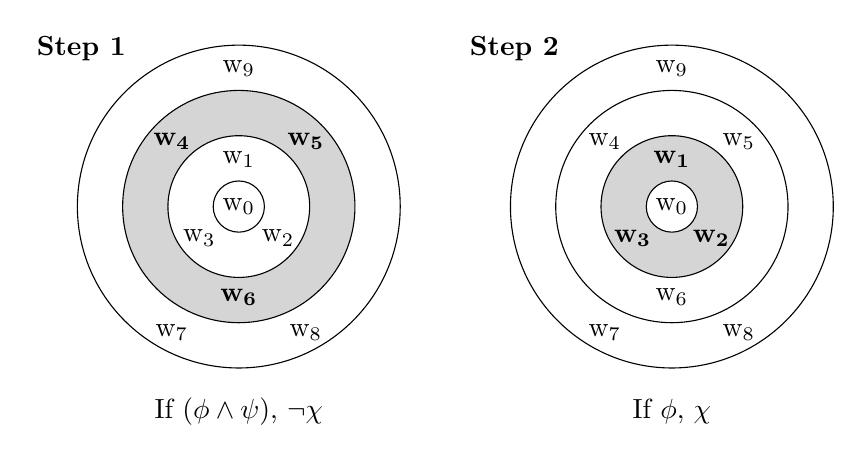
\begin{tikzpicture}
	\coordinate (O) at (0,0);
    \node at (-2,2) {\textbf{Step 1}};
	\draw[fill=white] (O) circle (2.05);
	\draw[fill=gray!33] (O) circle (1.475);
	\draw[fill=white] (O) circle (0.9);
	\draw[fill=white] (O) circle (0.325)node {w\textsubscript{0}};

	\node at (0,0.6) {w\textsubscript{1}};
	\node at (0.5,-0.4) {w\textsubscript{2}};
	\node at (-0.5,-0.4) {w\textsubscript{3}};
	
	\node at (-0.85,0.825) {\textbf{w\textsubscript{4}}};
	\node at (0.85,0.825) {\textbf{w\textsubscript{5}}};
	\node at (0,-1.15) {\textbf{w\textsubscript{6}}};
	
	\node at (-0.85,-1.6) {w\textsubscript{7}};
	\node at (0.85,-1.6) {w\textsubscript{8}};
	\node at (0,1.75) {w\textsubscript{9}};
	
	\node at (0,-2.6) {If $(\phi\land\psi)$, $\neg\chi$};
	
	
	\begin{scope}[xshift=5.5cm]
		\coordinate (O) at (0,0);
        \node at (-2,2) {\textbf{Step 2}};
    \draw[fill=white] (O) circle (2.05);
	\draw[fill=white] (O) circle (1.475);
	\draw[fill=gray!33] (O) circle (0.9);
	\draw[fill=white] (O) circle (0.325)node {w\textsubscript{0}};

	\node at (0,0.6) {\textbf{w\textsubscript{1}}};
	\node at (0.5,-0.4) {\textbf{w\textsubscript{2}}};
	\node at (-0.5,-0.4) {\textbf{w\textsubscript{3}}};
	
	\node at (-0.85,0.825) {w\textsubscript{4}};
	\node at (0.85,0.825) {w\textsubscript{5}};
	\node at (0,-1.15) {w\textsubscript{6}};
	
	\node at (-0.85,-1.6) {w\textsubscript{7}};
	\node at (0.85,-1.6) {w\textsubscript{8}};
	\node at (0,1.75) {w\textsubscript{9}};
	
	\node at (0,-2.6) {If $\phi$, $\chi$};
	\end{scope}
\end{tikzpicture}
\caption{Quantificational domains for reverse Sobel sequences according to \textcite{Stalnaker1968} and \citepos{Lewis1973} variably-strict conditional analyses. For all worlds $w_n$: If $n\geqslant1$, then $\phi=1$ is true for $w_n$, and if $n\geqslant 4$, then $\psi=1$ holds true for $w_n$. If $n\geqslant 7$, then some proposition $\omega=1$ such that $\omega\neq\phi$, $\omega\neq\psi$, and $\phi,\psi$ do not precede $\omega$ on some causal chain of events.}\labfig{stalnakerlewis-rSS}
\end{figure}

\noindent Since the sequence's two relevant domains of quantification are entirely disjoint, it makes---from a semantic point of view---no difference in which order a claim about the respective worlds is made. As such, it would falsely predict the reverse Sobel sequence's $\phi$-conditional to be felicitous.
\subsection{(Semi-)Dynamic Strict Semantics}
The infelicity of reverse Sobel sequences led to a return to the strict conditional analysis, as that approach correctly predicted the infelicity of such sequences. To also account for normal Sobel sequences, however, the original model required additional constraints on the domain of quantification, such that normal Sobel sequences do not yield a contradiction but that reverse Sobel sequences do. This led to the inception of the (semi-)dynamic strict conditional line of thought, as originally proposed by \textcite{Fintel2001} and \textcite{Gillies2007}. \textcite{Fintel2001} proposes that counterfactual conditionals are analysed as strict conditionals that range over a contextually determined domain of quantification. Counterfactual conditionals also come with an entertainability presupposition that their antecedents must be possible with respect to the aforementioned contextually set domain of quantification. If this presupposition is violated---that is, the contextually determined domain of quantification does not contain any world that the antecedent requires---then the contextual quantificational domain is expanded to encompass all possible worlds up to including the closest possible antecedent worlds. For this reason, \textcite{Fintel2001} also refers to the contextually-expanding domain of quantification as a modal horizon. This process is formally accomplished via the accessibility relation $f_\sigma$ as determined by the context $\sigma$ (which starts off as containing just the evaluation world itself). If the context does not contain any antecedent worlds, the counterfactual in question updates $\sigma$ such that $\sigma$ contains all worlds up to and including the closest antecedent worlds, as defined in \refdef{fintel}. The updated context is then kept for any subsequent counterfactual conditionals, with the process of updating $\sigma$ being reiterated if necessary.\vspace{-5mm}
\pex\phantomsection\labdef{fintel}\resizebox{395pt}{!}{\pextitle{Modal Horizon and Counterfactual Semantics by \citet{Fintel2001} for `If p, q'}}
\a\extitle{Context Change Potential}$f_\sigma+\intension[]{would}_{KvF}(q)(p)(w) = f^p_\sigma = [\lambda w_s.f_\sigma(w)\cup\{w':\forall w''\in p[w'\leqslant_w w'']\}]$
\a\extitle{Truth Conditions}$\intension[\sigma]{would}_{KvF}=[\lambda q_{<s,t>}.[\lambda p_{<s,t>}.[\lambda w_s.\hspace{1mm}\forall v\in f^p_\sigma(w)\cap p\hspace{0.5mm}[q(v)]\hspace{1mm}]]]$\vspace*{-2mm}
\xe
This process is illustrated in \reffig{fintel-contextchange} for the conditional \enquote{If p, q}.\vspace{-2mm}
\begin{figure}[!htb]
\resizebox{0.95\textwidth}{!}{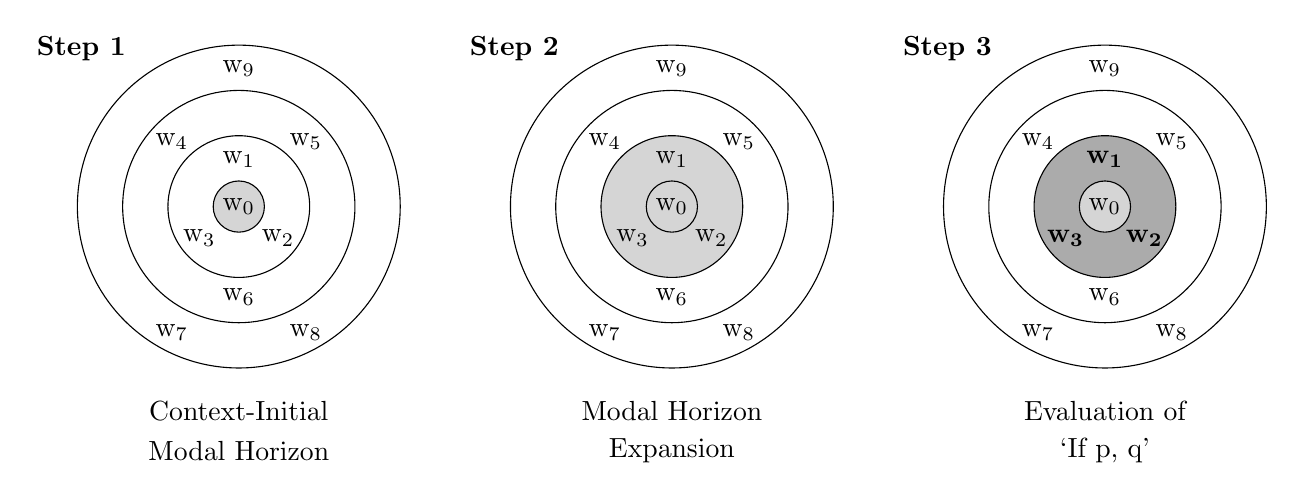
\begin{tikzpicture}
	\coordinate (O) at (0,0);
    \node at (-2,2) {\textbf{Step 1}};
	\draw[fill=white] (O) circle (2.05);
	\draw[fill=white] (O) circle (1.475);
	\draw[fill=white] (O) circle (0.9);
	\draw[fill=gray!33] (O) circle (0.325)node {w\textsubscript{0}};

	\node at (0,0.6) {w\textsubscript{1}};
	\node at (0.5,-0.4) {w\textsubscript{2}};
	\node at (-0.5,-0.4) {w\textsubscript{3}};
	
	\node at (-0.85,0.825) {w\textsubscript{4}};
	\node at (0.85,0.825) {w\textsubscript{5}};
	\node at (0,-1.15) {w\textsubscript{6}};
	
	\node at (-0.85,-1.6) {w\textsubscript{7}};
	\node at (0.85,-1.6) {w\textsubscript{8}};
	\node at (0,1.75) {w\textsubscript{9}};
	
	\node at (0,-2.6) {Context-Initial};
	\node at (0,-3.1) {Modal Horizon};
	
	
	\begin{scope}[xshift=5.5cm]
		\coordinate (O) at (0,0);
        \node at (-2,2) {\textbf{Step 2}};
    \draw[fill=white] (O) circle (2.05);
	\draw[fill=white] (O) circle (1.475);
	\draw[fill=gray!33] (O) circle (0.9);
	\draw[fill=gray!33] (O) circle (0.325)node {w\textsubscript{0}};

	\node at (0,0.6) {w\textsubscript{1}};
	\node at (0.5,-0.4) {w\textsubscript{2}};
	\node at (-0.5,-0.4) {w\textsubscript{3}};
	
	\node at (-0.85,0.825) {w\textsubscript{4}};
	\node at (0.85,0.825) {w\textsubscript{5}};
	\node at (0,-1.15) {w\textsubscript{6}};
	
	\node at (-0.85,-1.6) {w\textsubscript{7}};
	\node at (0.85,-1.6) {w\textsubscript{8}};
	\node at (0,1.75) {w\textsubscript{9}};
	
	\node at (0,-2.6) {Modal Horizon};
	\node at (0,-3.1) {Expansion};
	
	
	\begin{scope}[xshift=5.5cm]
		\coordinate (O) at (0,0);
        \node at (-2,2) {\textbf{Step 3}};
    \draw[fill=white] (O) circle (2.05);
	\draw[fill=white] (O) circle (1.475);
	\draw[fill=gray!66] (O) circle (0.9);
	\draw[fill=gray!33] (O) circle (0.325)node {w\textsubscript{0}};

	\node at (0,0.6) {\textbf{w\textsubscript{1}}};
	\node at (0.5,-0.4) {\textbf{w\textsubscript{2}}};
	\node at (-0.5,-0.4) {\textbf{w\textsubscript{3}}};
	
	\node at (-0.85,0.825) {w\textsubscript{4}};
	\node at (0.85,0.825) {w\textsubscript{5}};
	\node at (0,-1.15) {w\textsubscript{6}};
	
	\node at (-0.85,-1.6) {w\textsubscript{7}};
	\node at (0.85,-1.6) {w\textsubscript{8}};
	\node at (0,1.75) {w\textsubscript{9}};
	
	\node at (0,-2.6) {Evaluation of};
	\node at (0,-3.1) {`If p, q'};
	\end{scope}
	\end{scope}
	
\end{tikzpicture}}
\caption{Modal horizon (all shades of grey) and antecedent worlds quantified over (dark grey) for the conditional \enquote{If p, q}, according to \citepos{Fintel2001} semi-dynamic strict analysis, when the context initial modal horizon does not contain any suitable antecedent worlds. For all worlds $w_n$: If $n\geqslant1$, then $p=1$ is true for $w_n$.}\labfig{fintel-contextchange}
\end{figure}

For Sobel sequences, this means that the $\phi$-conditional updates $\sigma$ such that it contains all possible worlds up to including the closet $\phi$-worlds. Crucially, this means that the modal horizon does not contain any $\phi\land\psi$-worlds, since these worlds are less close to the evaluation world than the closet $\phi$-worlds. Since the $\phi\land\psi$-conditional's domain of quantification would then be empty, it further updates $\sigma$ to include the closest $\phi\land\psi$-worlds as as well. This way, the felicity of Sobel sequences would be explained, as illustrated in \reffig{fintel-SS}.
\begin{figure}[!htb]
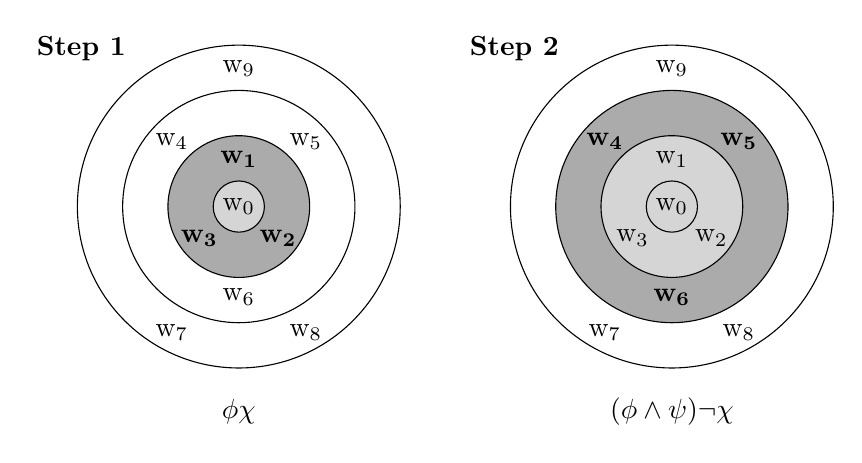
\begin{tikzpicture}
	\coordinate (O) at (0,0);
    \node at (-2,2) {\textbf{Step 1}};
	\draw[fill=white] (O) circle (2.05);
	\draw[fill=white] (O) circle (1.475);
	\draw[fill=gray!66] (O) circle (0.9);
	\draw[fill=gray!33] (O) circle (0.325)node {w\textsubscript{0}};

	\node at (0,0.6) {\textbf{w\textsubscript{1}}};
	\node at (0.5,-0.4) {\textbf{w\textsubscript{2}}};
	\node at (-0.5,-0.4) {\textbf{w\textsubscript{3}}};
	
	\node at (-0.85,0.825) {w\textsubscript{4}};
	\node at (0.85,0.825) {w\textsubscript{5}};
	\node at (0,-1.15) {w\textsubscript{6}};
	
	\node at (-0.85,-1.6) {w\textsubscript{7}};
	\node at (0.85,-1.6) {w\textsubscript{8}};
	\node at (0,1.75) {w\textsubscript{9}};
	
	\node at (0,-2.6) {$\phi\cf\chi$};
	
	
	\begin{scope}[xshift=5.5cm]
		\coordinate (O) at (0,0);
        \node at (-2,2) {\textbf{Step 2}};
    \draw[fill=white] (O) circle (2.05);
	\draw[fill=gray!66] (O) circle (1.475);
	\draw[fill=gray!33] (O) circle (0.9);
	\draw[fill=gray!33] (O) circle (0.325)node {w\textsubscript{0}};

	\node at (0,0.6) {{w\textsubscript{1}}};
	\node at (0.5,-0.4) {{w\textsubscript{2}}};
	\node at (-0.5,-0.4) {{w\textsubscript{3}}};
	
	\node at (-0.85,0.825) {\textbf{w\textsubscript{4}}};
	\node at (0.85,0.825) {\textbf{w\textsubscript{5}}};
	\node at (0,-1.15) {\textbf{w\textsubscript{6}}};
	
	\node at (-0.85,-1.6) {w\textsubscript{7}};
	\node at (0.85,-1.6) {w\textsubscript{8}};
	\node at (0,1.75) {w\textsubscript{9}};
	
	\node at (0,-2.6) {$(\phi\land\psi)\cf\neg\chi$};
	\end{scope}
\end{tikzpicture}
\caption{Quantificational domains for Sobel sequences according to \citepos{Fintel2001} semi-dynamic strict conditional analysis. For all worlds $w_n$: If $n\geqslant1$, then $\phi=1$ is true for $w_n$, and if $n\geqslant 4$, then $\psi=1$ holds true for $w_n$. Non-antecedent worlds present within the modal horizon are shaded in the lighter grey.}\labfig{fintel-SS}
\end{figure}

For reverse Sobel sequences, the situation is slightly different. The initial $\phi\land\psi$-conditional update $\sigma$ to include all possible worlds of similarity equal to or greater than the closest $\phi\land\psi$-worlds. Naturally, this also includes the closest $\phi$-worlds. 

The subsequent $\phi$-conditional's domain of quantification already contains some antecedent worlds and, as such, does not require an expansion of the modal horizon. Neither does the modal horizon contract to exclude any semantically unnecessary worlds. The $\phi$-conditional would therefore quantify not only over the closest $\phi$-worlds, but any other $\phi$-worlds already present in the context, including the closest $\phi\land\psi$-worlds. This would obviously contradict the meaning of the previous $\phi\land\psi$-conditional, thereby deriving the infelicity of reverse Sobel sequences, as illustrated in \reffig{fintel-rSS}.
\begin{figure}[!htb]
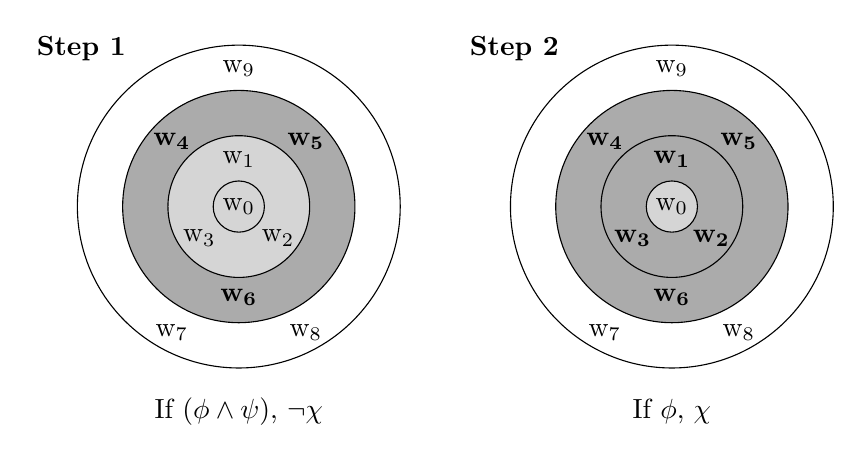
\begin{tikzpicture}
	\coordinate (O) at (0,0);
    \node at (-2,2) {\textbf{Step 1}};
	\draw[fill=white] (O) circle (2.05);
	\draw[fill=gray!66] (O) circle (1.475);
	\draw[fill=gray!33] (O) circle (0.9);
	\draw[fill=gray!33] (O) circle (0.325)node {w\textsubscript{0}};

	\node at (0,0.6) {{w\textsubscript{1}}};
	\node at (0.5,-0.4) {{w\textsubscript{2}}};
	\node at (-0.5,-0.4) {{w\textsubscript{3}}};
	
	\node at (-0.85,0.825) {\textbf{w\textsubscript{4}}};
	\node at (0.85,0.825) {\textbf{w\textsubscript{5}}};
	\node at (0,-1.15) {\textbf{w\textsubscript{6}}};
	
	\node at (-0.85,-1.6) {w\textsubscript{7}};
	\node at (0.85,-1.6) {w\textsubscript{8}};
	\node at (0,1.75) {w\textsubscript{9}};
	
	\node at (0,-2.6) {If $(\phi\land\psi)$, $\neg\chi$};
	
	
	\begin{scope}[xshift=5.5cm]
		\coordinate (O) at (0,0);
        \node at (-2,2) {\textbf{Step 2}};
    \draw[fill=white] (O) circle (2.05);
	\draw[fill=gray!66] (O) circle (1.475);
	\draw[fill=gray!66] (O) circle (0.9);
	\draw[fill=gray!33] (O) circle (0.325)node {w\textsubscript{0}};

	\node at (0,0.6) {\textbf{w\textsubscript{1}}};
	\node at (0.5,-0.4) {\textbf{w\textsubscript{2}}};
	\node at (-0.5,-0.4) {\textbf{w\textsubscript{3}}};
	
	\node at (-0.85,0.825) {\textbf{w\textsubscript{4}}};
	\node at (0.85,0.825) {\textbf{w\textsubscript{5}}};
	\node at (0,-1.15) {\textbf{w\textsubscript{6}}};
	
	\node at (-0.85,-1.6) {w\textsubscript{7}};
	\node at (0.85,-1.6) {w\textsubscript{8}};
	\node at (0,1.75) {w\textsubscript{9}};
	
	\node at (0,-2.6) {If $\phi$, $\chi$};
	\end{scope}
\end{tikzpicture}
\caption{Quantificational domains for reverse Sobel sequences according to \citepos{Fintel2001} semi-dynamic strict conditional analysis. For all worlds $w_n$: If $n\geqslant1$, then $\phi=1$ is true for $w_n$, and if $n\geqslant 4$, then $\psi=1$ holds true for $w_n$. Non-antecedent worlds present within the modal horizon are shaded in the lighter grey.}\labfig{fintel-rSS}
\end{figure}

\citepos{Gillies2007} model of conditionals is very similar to \citepos{Fintel2001}. His model, however, is fully dynamic and goes on to explain why possibility modals also appear to expand the modal horizon, as is seen in Hegel sequences such as \refex{hegel}:
\ex\phantomsection\labex{hegel} If Sophie had gone to the parade, she would have seen Pedro dance;
but, of course, if Sophie had gone to the parade, she might have been stuck behind
someone tall and then wouldn’t have seen Pedro dance.\hfill\parencite[p. 342]{Gillies2007}
\xe
\section{Klecha (2014) -- Sobel Sequences and Causality}\labsec{sobelklecha}
Whilst the traditional narrative was one of general reverse Sobel sequence infelicity, subsequent research has shown that this sense of infelicity is far from universally applicable. Below are example reverse Sobel sequences that were judged as felicitous:
\ex\phantomsection\labex{ice}\context{Said to someone who had just been completely alone by a frozen lake.} If you had walked on the thin ice while being supported by someone on the shore, the ice wouldn't have broken. But, of course, if you had walked on the thin ice, the ice would have broken.\\%
\emptyfill(adapted from \textcite[p. 166]{Bennett2003} by \textcite[p. 488]{Lewis2018})
\xe
\ex\phantomsection\labex{match}\context{Holding up a dry match, with no water around.}If I had struck this match and it had been soaked, it would not have lit. But if I had struck this match, it would have lit.\\%
\emptyfill(adapted from \textcite[p. 106]{Stalnaker1968} by \textcite[p. 487]{Lewis2018})
\xe
Whilst the conditions under which reverse Sobel sequences are interpreted felicitously are not perfectly known, \textcite{Klecha2014,Klecha2015} provided one major step towards unmuddling this issue. He maintains that two independent phenomena have mistakenly been grouped together under the term of Sobel sequences: acausal Sobel sequences and causal Sobel sequences.\footnote{Originally, \textcite{Klecha2014}, referred to acausal Sobel sequences as Unequivocal Sobel sequences and to causal Sobel sequences as Equivocal Sobel sequences. Later on, \textcite{Klecha2015} respectively refers to these phenomena as True Sobel sequences and Lewis sequences to more clearly illustrate that he considers them to be entirely independent phenomena. For the sake of terminological transparency, we refer to these phenomena as acausal and causal Sobel sequences, respectively.} 

The first type, acausal Sobel sequences, exhibits two distinct properties: non-unidirectionality and unequivocality. Non-unidirectionality refers to the observation that acausal Sobel sequences are principally felicitously reversible (i.e., they are felicitous in either direction). The latter refers to the observation that acausal Sobel sequences generally constitute \enquote{a single pointful piece of discourse}, as put by \textcite{Edgington1995}; in other words, the speaker of a (reverse) acausal Sobel sequence does not appear to change their mind mid-sequence.

The second type, causal Sobel sequences, on the other hand, displays the opposite qualities: unidirectionality and equivocality. Unidirectionality refers to the observation that reverse causal Sobel sequences are infelicitous, even if their regularly ordered counterpart is felicitous. Equivocality refers to the observation that the speaker of a causal Sobel sequence appears to change their mind mid-sequence (e.g., upon noticing a hereto disregarded possible scenario that may falsify the $\phi$-conditional's consequent). 

The defining characteristic between them is that acausal Sobel sequences' $\phi$-conditionals are strengthened with a causally unrelated proposition $\psi$ to yield the $\phi\land\psi$-conditional, whereas, for causal Sobel sequences, $\phi$ and $\psi$ are causally related such that $\phi$ precedes $\psi$ on some causal chain of events. The difference in antecedental intracausal dependency and the resulting difference in unidirectionality is most easily demonstrated with the examples \refex{klecha1} and \refex{klecha2}, where \refex{klecha1} presents a (reverse) acausal Sobel sequence and \refex{klecha2} a (reverse) causal Sobel sequence:\footnote{Note that these examples are not pure reverse causal and acausal Sobel sequences. Rather, they are reverse Sobel sequences that overlap with their regular Sobel sequence counterpart. This was done by \textcite{Klecha2014} to create a minimal pair whilst avoiding a possible source of infelicity for acausal reverse Sobel sequence. This is further elaborated upon in \refsec{ASS}. But native speakers that I have consulted also find the following plain minimal pair acceptable, if appropriately stressed:\vspace{0mm}
\ex[exno=i] \phantomsection\contextpex{Concerning a dry match being displayed.}\\\speaker{S}If I had struck this match and it had been wet, it would not have lit; but if I \MakeUppercase{had} struck this match, it would have lit.
\xe%
\ex[exno=ii] \phantomsection\contextpex{Concerning a dry match being displayed.}\\\speaker{S}If I had struck this match and it had snapped, it would not have lit; \#but if I \MakeUppercase{had} struck this match, it would have lit.
\xe}\\
\pex\phantomsection\labex{klecha1}%
\contextpex{Construction workers Daryl, Aaron, and Ida, stand around a construction site.  Daryl is not wearing a helmet.  A large beam falls from above them and lands where no one was standing, but near to Daryl.}
			\a	\speaker{Aaron}Daryl, if you had been standing there, you would have been killed.
			\a	\speaker{Ida}But if he had been standing there and wearing a helmet, you would not have.
			\a	\speaker{Aaron}Exactly. But what I said is still right:  If you had been
standing there, you would have been killed.\hfill\parencite[p. 152f]{Klecha2014}
\xe
\pex\phantomsection\labex{klecha2}%
\contextpex{Construction workers Daryl, Aaron, and Ida, stand around a construction site.  Daryl is not wearing a helmet.  A large beam falls from above them and lands where no one was standing, but near to Daryl.}
			\a	\speaker{Aaron}Daryl, if you had been standing there, you would have been killed.
			\a	\speaker{Ida}But if he had been standing there and he saw the shadow of the falling beam and managed to jump out of the way in time, he would not have.
			\a	\speaker{Aaron}\#Exactly. But what I said is still right:  If you had been
standing there, you would have been killed.\hfill\parencite[adapted from][p. 153f]{Klecha2014}
\xe
In \refex{klecha1}, $\phi$ and $\psi$ are causally unrelated since Daryl wearing a helmet is in no obvious way connected to him standing where the steel beam had fallen. In \refex{klecha2}, they are causally connected, as him jumping out of the way in time is causally dependent on him standing where the steel beam had fallen. Both examples also perfectly illustrate the difference in equivocality. In \refex{klecha1}, both parties appear to argue in favour of the same point: Daryl should be wearing his helmet. This can be seen when Aaron agrees with Ida's argument that Daryl would have survived in the case of him having worn a helmet. It becomes even clearer, if the reaffirmation of the $\phi$-conditional is removed:\\\begin{minipage}{\linewidth}
\pex\phantomsection\labex{klecha1-exactly}%
\contextpex{Construction workers Daryl, Aaron, and Ida, stand around a construction site.  Daryl is not wearing a helmet.  A large beam falls from above them and lands where no one was standing, but near to Daryl.}
			\a	\speaker{Aaron}Daryl, if you had been standing there, you would have been killed.
			\a	\speaker{Ida}And if you had been standing there and wearing a helmet, you would not have.
			\a	\speaker{Aaron}Exactly.\hfill\parencite[p. 150]{Klecha2015}
\xe\end{minipage}
In \refex{klecha2}, on the other hand, Aaron and Ida appear to argue in favour of contrary positions: Aaron believes that Daryl would have died, had he stood at crash site, whereas Ida disputes that outcome with an alternative scenario. In a similar fashion of how removing the reaffirmation of the $\phi$-conditional more clearly demonstrates the unequivocality of the acausal Sobel sequence, does the removal of aforementioned affirmation clarify the equivocal nature of the causal Sobel sequence:
\pex\phantomsection\labex{klecha2-exactly}%
\contextpex{Construction workers Daryl, Aaron, and Ida, stand around a construction site.  Daryl is not wearing a helmet.  A large beam falls from above them and lands where no one was standing, but near to Daryl.}
			\a	\speaker{Aaron}Daryl, if you had been standing there, you would have been killed.
			\a	\speaker{Ida}But if he had been standing there and he saw the shadow of the falling beam and managed to jump out of the way in time, he would not have.
			\a	\speaker{Aaron}\#Exactly.\hfill\parencite[p. 153f]{Klecha2015}
\xe
The difference in unidirectionality is also adequately demonstrated with \refex{klecha1} and \refex{klecha2}. There is one important caveat concerning acausal Sobel sequences according to Klecha, however: Acausal Sobel sequences are in and of themselves reversible, but that does not mean that reverse acausal Sobel sequences are actually felicitous in every context, as demonstrated below.
\pex\phantomsection\labex{klecha-infelicitous}%
\contextpex{Construction workers Daryl, Aaron, and Ida, stand around a construction site.  Daryl is not wearing a helmet.  A large beam falls from above them and lands where no one was standing, but near to Daryl.}
\a\phantomsection\speaker{Ida}If you had been standing there and wearing a helmet, you
wouldn’t have been killed.
\a\phantomsection\speaker{Aaron}\#But if you had been standing there, you would have
been killed.\\\emptyfill\parencite[p. 151]{Klecha2014}
\xe
In summary, \textcite{Klecha2014} tries to account for the empirical distribution in \reftab{yetanotherfriggintable}.
\begin{table}[!htb]
\caption{Empirical Data of \textcite{Klecha2014} concerning Sobel sequences.}
\labtab{yetanotherfriggintable}
    \begin{tabular}{lcc}
    \toprule
                &   Causally Unrelated    &   Causally Related\\\midrule
          Regular Order    &   \checkmark  &   \checkmark\\
          Reverse Order   &   \checkmark,\#  &   \#\\
          \bottomrule
    \end{tabular}
\end{table}

\noindent As such, there are two contrasts that currently need to be accounted for: (i) The difference in felicity between causal and acausal reverse Sobel sequence and (ii) the difference in felicity between some reverse acausal Sobel sequences. For the former, we provide \citepos{Klecha2014,Klecha2015} account in \refsec{ASS} and \refsec{CSS}. For the latter, we provide \citepos{Klecha2014,Klecha2015} attempt at an explanation in \refsec{ASS}.
\subsection{Acausal Sobel Sequences}\labsec{ASS}
Without any special intonation, the reverse acausal Sobel sequence in \refex{klecha-infelicitous} is generally considered infelicitous. \textcite[p. 151f]{Klecha2014} argues that the infelicity of infelicitous reverse acausal Sobel sequences can be ascribed to two possible sources: First, it is possible that \textit{would} is susceptible to modal subordination and the \textit{would} of the $\phi$-conditional is therefore interpreted not with respect to just $\phi$ but with respect to $\phi\land(\phi\land\psi)$, causing a contradictory reading. Second, it is possible that the $\phi$-conditional is infelicitous simply due to the fact that there is some pressure to stress its antecedent contrastively against the antecedent of the preceding $\phi\land\psi$-conditional. In cases where the $\phi$-conditional's antecedent happens to be a syntactic subset of the $\phi\land\psi$-conditional, as is the case in \refex{klecha-infelicitous}, \textcite{Klecha2014,Klecha2015} argues that this cannot be done, which therefore automatically renders the reverse acausal Sobel sequence infelicitous.\footnote{It should be noted that \parencite{Klecha2014,Klecha2015} does not explain why this ceases to be the case once the reverse acausal Sobel sequence is overlapped with its regularly ordered counterpart, as in \refex{klecha1}.} If, however, there is some element in the $\phi$-conditional's antecedent that is overtly different from the $\phi\land\psi$-conditional's counterpart, then that element is obligatorily stressed, resulting in felicity. An example of this is provided by the reverse Sobel sequence in \refex{contrast-host}, below.\footnote{Note that \refex{contrast-host} is a reverse Sobel sequence due to its sentences being interpreted as \textit{If Karlos had come to the party} and as \textit{If Karlos had come to and hosted the party}, where \textit{come to} is interpreted along the lines of being present, rather than it being an active act of Karlos that requires him to go somewhere that is not his own home. As such, Karlos hosting the party would entail Karlos coming to the party.}
\pex[nopreamble=true]\phantomsection\label{ex:contrast-host}%
\a\phantomsection\speaker{Ben}If Karlos had hosted the party, it would not have been a good time.
\a\phantomsection\speaker{Martina}But if Karlos had \MakeUppercase{come} to the party, it would have been a good time.\hfill\parencite[p.~151]{Klecha2014}
\xe
Since it could be argued that this sequence's $\phi$-conditional carries an exhaustive reading (in the sense of \textit{Karlos had come but not hosted the party}), which may be responsible for the sequence's felicity, \textcite{Klecha2014} goes on to argue that this concern can be alleviated by overlapping the reverse acausal Sobel sequence with its regularly ordered counterpart, as seen below, which should prevent this particular reading. 
\pex\phantomsection%
\contextpex{Karlos is known for being fun at parties. But his house is small and smelly.}
\a\phantomsection\speaker{Martina}If Karlos had come to the party, it would have been a good time.
\a\phantomsection\speaker{Ben}But if Karlos had hosted the party, it would not have been a good time.
\a\phantomsection\speaker{Martina}Sure, but what I said is still right: If Karlos had come
to the party, it would have been a good time.
\xe
However, the generalisation that contrastive stress is only possible if the second antecedent is not a subset of the first one is not entirely correct. We have already seen examples of reverse acausal Sobel sequences that do not fulfil this requirement yet still remain felicitous. An example of this would be \refex{match}, repeated below as \refex{match-repeat}, modified to indicate stress placement in the second antecedent.
\ex\phantomsection\labex{match-repeat}\context{Holding up a dry match, with no water around.}If I had struck this match and it had been soaked, it would not have lit. But if I \MakeUppercase{had} struck this match, it would have lit.\\%
\emptyfill(adapted from \textcite[p. 106]{Stalnaker1968} by \textcite[p. 487]{Lewis2018})
\xe
In cases where there is no overtly different lexical item to be found, the required stress appears to obligatorily fall upon the auxiliary verb, should the conditional sequence contain any.\footnote{Note that we explore the question of whether or not this stress on the auxiliary verb is also an instance of contrastive focus/stress in \refch{pragmatics-SS}. For the sake of this chapter, we just group both types of stress together.} As such, we must amend our current empirical data on (reverse) Sobel sequences to reflect this previously unnoticed fact:
\begin{table}[!htb]
\caption{Current empirical data on (reverse) Sobel sequences broken down by the factors of causality and the second antecedent being a subset of the first antecedent.}
\begin{tabular}{lcccc}
    \toprule
                &   \multicolumn{2}{c}{Causally Unrelated}    &   \multicolumn{2}{c}{Causally Related}\\
                &   Syntactic Subset  &   Not Syntactic Subset  \\\midrule
          Regular Order &   \checkmark  &   \checkmark  &   \multicolumn{2}{c}{\checkmark}\\
          Reverse Order &   \#, \checkmark  &   \checkmark          &   \multicolumn{2}{c}{\#}\\
          \bottomrule
    \end{tabular}
\end{table}

Critically, \textcite{Klecha2014,Klecha2015} does not motivate (i) why contrastive stress is needed, and (ii) why only some reverse acausal Sobel sequences undergo modal subordination. As such, these parts of his analysis are more akin to possible factors or approaches, rather than a fully-fledged account of reverse acausal Sobel sequence infelicity, as he himself admitted. We further explore these issues in \refch{pragmatics-SS}, motivating the need for contrastive stress, systematising its effects, and linking it to causality such that the difference in felicity between causal and acausal reverse Sobel sequences follows naturally from our analysis.

\subsection{Causal Sobel Sequences and Imprecision}\labsec{CSS}
Concerning causal Sobel sequences, \textcite{Klecha2014,Klecha2015} argues that their unidirectionality is directly linked to the more well-known phenomenon of imprecision and precisification.
We follow \citepos{Klecha2014} analysis of imprecision, which was built upon the ideas and analyses of \textcite{Lasersohn1999}, \textcite{Krifka2009}, and \textcite{Lauer2012}.

\subsubsection{Imprecision and Precisification}
As \textcite[p. 352ff]{Lewis1979} has pointed out, we are allowed to utter---and evaluate as true---notions that are strictly considered objectively false, so long as these notions are \enquote{true enough} for the current discourse purpose. Consider the following examples:
\pex[nopreamble=true]\phantomsection%
\a\phantomsection\phantomsection France is hexagonal\hfill\parencite[p. 142]{Austin1976}\labex{france}
\a\phantomsection\phantomsection This table is flat.\labex{table}\xe
The sentence in \refex{france}, for example, is strictly speaking false, yet may be considered roughly true (i.e., \textit{true enough} to use \citepos{Lewis1979} terminology) for simple discussions on the shape of France. For discussions between cartographers, however, this statement would be evaluated as false---as it does not live up to the standards of precision expected from a discussion between cartographers \parencite[p. 142]{Austin1976}. Yet the sentence in \refex{table} would be considered true in nearly all feasible contexts (assuming that the table in question appears flat to the human eye), despite the fact that no man-made construct could ever be truly flat down to the molecular level \parencite[for details, see][]{Unger1975}. This shows that any discourse is subject to differing levels of precision---a crucial component of the \enquote{conversational score}, as argued by \textcite{Lewis1979}. Whether sentences such as \refex{france} and \refex{table} are evaluated as false or as true depends entirely upon which level of precision is set for the discourse in question. However, contrary to the other elements of the conversational score, the level of precision of any given discourse may fluctuate depending on the individual discourse moves it consists of. See below for an example:
\pex\phantomsection\labex{flat}%
\contextpex{Katie and Lelia stand around a table made by humans.}
\a\phantomsection\speaker{Katie}This table is flat.\hfill{\scshape loose claim}
\a\phantomsection\speaker{Lelia}Not really. Nothing made by humans is actually flat.\hfill{\scshape rebuttal}
\a\phantomsection\labex{flat-concession}\speaker{Katie}Well, okay, whatever. But you get my drift.\hfill{\scshape concession}\\
\emptyfill\parencite[p. 113]{Klecha2014}
\xe
In \refex{flat}, Lelia elevates the level of precision and validly (though pedantically) disclaims Katie's previously true-enough proposition as false. The act of raising the level of precision is referred to as precisification. \textcite[p. 114]{Klecha2014} ascribes to speech acts such as the one in \refex{flat} three common properties: (i) pedantry, (ii) inessential disagreement, and (iii) unidirectionality.

\textit{Pedantry} is defined as \enquote{a kind of intuition of mild uncooperativity} \parencite[p. 114]{Klecha2014}. Whilst Lelia's rebuttal is not entirely appropriate for most possible discourse contexts, it is also not totally inappropriate: Her unnecessary and unwarranted attempt at precisification and falsification may cause feelings of annoyance, it appears to not reach levels of uncooperativity as, for example, intentionally misinterpreting Katie's statement. \textcite{Klecha2014} demonstrated this by contrasting \refex{flat} with \refex{flat-beer}:
\pex\phantomsection\labex{flat-beer}%
\contextpex{Katie and Lelia stand around a table made by humans.}\a\phantomsection\speaker{Katie}This table is flat.
\a\phantomsection\speaker{Lelia}\#Well sure, but have you ever seen a carbonated table?
\a\phantomsection\speaker{Katie}What are you talking about? I meant \MakeUppercase{flat} like \MakeUppercase{level}.\\\emptyfill\parencite[p. 114]{Klecha2014}
\xe
Here, the insane interpretation of Lelia of \textit{flat} to mean decarbonated---an attribute that is only typically applied to drinks such as beer---is simply infelicitous rather than only being a pedantic interjection.

\textit{Inessential Disagreement} is similar to faultless disagreement---typical of predicates expressing personal tastes and opinions, as seen in \refex{taste}---but, contrary to faultless disagreement, incorporates a sense of concession without actually changing ones opinion (i.e., a partial concession). In \refex{flat-concession}, the reluctance and defence of Katie's original position shows that she does not think that she is mistaken about the facts or willing to change her mind, but she acknowledges the truth of Lelia's statement, given a higher level of precision. This is opposite to faultless disagreement where the same discourse moves would seemingly involve changing ones mind and a sense of infelicity when it comes to the defence.\enlargethispage*{2\baselineskip}

\pex\phantomsection\labex{taste}%
\contextpex{Raphael and Sterling eat a meal together.}\a\phantomsection\speaker{Raphael}This is delicious.
\a\phantomsection\speaker{Sterling}No it isn’t.
\a\phantomsection\speaker{Raphael}?Well, okay, whatever. ??But you get my drift.\\\emptyfill\parencite[adapted from][p. 114]{Klecha2014}
\xe
As such, \textit{partial concession} is considered a diagnostic of inessential disagreement.

\textit{Unidirectionality}---or irreverisibility in the case of Sobel sequences---refers to the fact that levels of precision are far more easily increased than decreased \parencite{Lewis1979}: Discourse participants typically have to go along with whatever increase in precision has been introduced to the discourse, as previously seen in \refex{flat}, whereas implicit attempts to lower the standard of precision are ignored and any associated loose talk is evaluated with respect to the higher standard of precision in the discourse:
\pex\phantomsection\labex{flat-reverse}%
\contextpex{Katie and Lelia stand around a table made by humans.}
\a\phantomsection\speaker{Lelia}This table's surface is tilted by almost one tenth of a degree and contains a number of wooden bumps that are a few micrometers in height.\\\emptyfill{\scshape precise claim}
\a\phantomsection\speaker{Katie}\#This table is flat.\hfill{\scshape loose claim}
\xe

\subsubsection{Imprecision and Its Relation to Causal Sobel Sequences}\labsec{css-bennett-explanation}
\textcite{Klecha2014} argues that (i) imprecision is required for the consistent evaluation of causal Sobel sequences and (ii) that the unidirectional nature of precisification is directly responsible for the infelicity of reverse causal Sobel sequences. This follows from his adoption of \citepos{Bennett2003} view on how causality affects world closeness.

\textcite{Bennett2003} argues that the closeness of some world $w$ to the evaluation world $w_0$ is not decreased or increased by any differences that causally followed from some initial difference to the evaluation world. In other words: \textcite{Bennett2003} argues that the closeness metric is indifferent to any dissimilarity that follows from the antecedent on some causal chain of events. As such, when it comes to calculating the world closeness ordering, only the initial antecedent and matters causally unrelated to the antecedent affect the closeness of worlds. 

\textcite{Bennett2003} provides motivation in the form of the following argument: If every kind of dissimilarity between worlds were to affect world closeness, then, for counterfactual conditionals, the set of closest antecedent worlds would typically consist of worlds that are near-totally identical to the evaluation world, excepting the proposition of the antecedent itself. This is especially problematic for changes that are likely to yield large-scale differences to the evaluation world. Take the 2016 US presidential election and its counterfactual possibilities for example:\vskip -2.25mm
\ex\phantomsection\labex{hillary}If Hillary had won the US election, the USA would not have alienated the majority of its allies and would have remained a global diplomatic superpower.\xe\vskip -2.25mm
\noindent The counterfactual in \refex{hillary} would quantify over the closest antecedent worlds in which Hillary won the election and check whether the consequent applies to these worlds. However, a na\"ive similarity implementation \`a la \textcite{Lewis1973} would suggest that these closest worlds are actually worlds in which Hillary is a male Republican that shares most if not all of the rhetoric and policies of Donald Trump---as such worlds would arguably contain fewer dissimilarities to our current actual world. If, however, only those dissimilarities that are causally unrelated to the antecedent decrease world closeness, then any Trump-esque Hillary Clinton worlds would be considered rather remote to the actual world, as any such a change to the entity \textit{Hillary Clinton} would be causally unrelated to the antecedent, thereby decreasing world closeness. Any worlds where Hillary Clinton acted in accordance with her character as a female US democrat, on the other hand, would causally follow from the antecedent and therefore not decrease world closeness, regardless of how vastly different these acts would be to Trump's or how great the impact of these acts would be. As such, \refex{hillary} would definitely be evaluated as false by a na\"ive implementation of \textcite{Lewis1973}, but would probably evaluated as true by \textcite{Bennett2003}, since his implementation disregards the dissimilarity of events causally related to the antecedent.\footnote{Naturally, this evaluation depends upon the expectations people have concerning how Hillary Clinton would have acted as president of the USA, and, as such, may differ from reader to reader.}

This also directly leads us to the problem of regular causal Sobel sequences and the standard Lewisian variably-strict account: Causal Sobel sequences' antecedents are, by definition, such that $\psi$ follows from $\phi$ on some causal chain of events. As such, \textcite{Bennett2003} would argue that the closest $\phi\land\psi$-worlds are a subset of the closest $\phi$-worlds (i.e. both sets of worlds are equal in closeness to the evaluation world). This would yield a contradictory reading where we first claim that all the closest $\phi$-worlds are $\chi$-worlds, and then claim that some of these $phi$-worlds (namely the $\phi\land\psi$-worlds) are actually not $\chi$-worlds after all. 

\textcite{Klecha2014} circumvents this contradictory reading via the introduction of imprecision: The causal Sobel sequence's $\phi$-conditional is a form of loose talk, where the closest $\phi\land\psi$-worlds are omitted from the world closeness ordering due to prevailing low standards of precision. This leaves the $\phi$-conditional to quantify over only the closest $\phi$-worlds that are not also $\phi\land\psi$-worlds. The $\phi\land\psi$-conditional then raises the level of precision to include the $\phi\land\psi$-worlds in the world closeness ordering, allowing it to quantify over these worlds. In other words, the evaluation of the $\phi\land\psi$-worlds necessitates precisification.

Conversely, \textcite{Klecha2014} explains the irreversibility of causal Sobel sequences via the unidirectional nature of precisification. For reverse causal Sobel sequences, the utterance of the $\phi\land\psi$-conditional already raises the level of precision such that the closest $\phi\land\psi$-worlds are available for evaluation. Since precisification is largely unidirectional, as demonstrated in \refex{flat-reverse}, the subsequent $\phi$-conditional is forced to maintain the same degree of precision when it comes to its evaluation, resulting in the closest $\phi$-worlds containing all of the closest $\phi\land\psi$-worlds. This would yield a contradictory reading, deriving the general infelicity of reverse causal Sobel sequences.

\textcite{Klecha2014} argues in favour of imprecision due to the parallels between regular precisification examples, as in \refex{table-imprecision} and (reverse) causal Sobel sequences, as in \refex{klecha2}, repeated below as \refex{klecha2-repeat}. For instance, both disallow any repetition of the original utterance after some (precisifying) rebuttal and thus prevent the original speaker from maintaining their original belief without concessions:%
\pex\phantomsection\labex{table-imprecision}%
\contextpex{Katie and Lelia stand around a table made by humans.}\vspace{-2mm}
\a\phantomsection\speaker{Katie}This table is flat.
\a\phantomsection\speaker{Lelia}Not really. Nothing made by humans is actually flat.
\a\phantomsection\speaker{Katie}\#Exactly. But what I said is still right: This table is flat.\\
\emptyfill\parencite[adapted from][p. 113]{Klecha2014}
\xe
\pex\phantomsection\labex{klecha2-repeat}%
\contextpex{Construction workers Daryl, Aaron, and Ida, stand around a construction site.  Daryl is not wearing a helmet.  A large beam falls from above them and lands where no one was standing, but near to Daryl.}
			\a	\speaker{Aaron}Daryl, if you had been standing there, you would have been killed.
			\a	\speaker{Ida}But if he had been standing there and he saw the shadow of the falling beam and managed to jump out of the way in time, he would not have.
			\a	\speaker{Aaron}\#Exactly. But what I said is still right:  If you had been
standing there, you would have been killed.\hfill\parencite[adapted from][p. 153f]{Klecha2014}
\xe
Both phenomena, however, allow for partial concessions, insofar as that the original asserter acknowledges the rebuttal but maintains the underlying motivation behind their original assertion, as shown in \refex{flat}---repeated below as \refex{flat-zzz}---and \refex{moreklechastuffzzz}.
\pex\phantomsection\labex{flat-zzz}%
\contextpex{Katie and Lelia stand around a table made by humans.}
\a\phantomsection\speaker{Katie}This table is flat.\hfill{\scshape loose claim}
\a\phantomsection\speaker{Lelia}Not really. Nothing made by humans is actually flat.\hfill{\scshape rebuttal}
\a\phantomsection\speaker{Katie}Well, okay, whatever. But you get my drift.\hfill{\scshape concession}\\
\emptyfill\parencite[p. 113]{Klecha2014}
\xe
\pex\phantomsection\labex{moreklechastuffzzz}%
\contextpex{Construction workers Daryl, Aaron, and Ida, stand around a construction site.  Daryl is not wearing a helmet.  A large beam falls from above them and lands where no one was standing, but near to Daryl.}
			\a	\speaker{Aaron}Daryl, if you had been standing there, you would have been killed.
			\a	\speaker{Ida}But if he had been standing there and he saw the shadow of the falling beam and managed to jump out of the way in time, he would not have.
			\a	\speaker{Aaron}Well, okay, whatever. But you get my drift: It's not safe, so he should really be wearing a helmet.
\xe


\subsubsection{Observation Regarding Reversibility}\labsec{klecha-no}
However, not all data points towards causal Sobel sequences being entirely unidirectional: As seen in \refex{rLS-felicitous}, reverse causal Sobel sequences are felicitous, if an interjection between the $\phi\land\psi$-conditional and the $\phi$-conditional denigrates the relevance or probability of the closest $\phi\land\psi$-worlds, the $\phi$-conditional may be uttered felicitously: 
\pex\phantomsection\labex{rLS-felicitous}%
\contextpex{Construction workers Daryl, Aaron, and Ida, stand around a construction site.  Daryl is not wearing a helmet.  A large beam falls from above them and lands where no one was standing, but near to Daryl. Daryl is also known to possess exceptionally bad reflexes: Generally, nine out of ten attempts to evade something as fast as the falling steel beam result in failure.}
	\a	\speaker{Aaron}Daryl, if you had been standing there, you would have been killed.
	\a\phantomsection\labex{rLS-felicitous-phipsi}\speaker{Ida}But if he had been standing there and he saw the shadow of the falling beam and managed to jump out of the way in time, he would not have.
	\a\phantomsection\labex{rLS-felicitous-psi2}\speaker{Aaron}Sure, that may be possible, but the chances of that happening are like really, really low. So, my point stands: If he had stood there, he would have died.\hfill\parencite[adapted and modified from][p. 134]{Klecha2014}
\xe
At first glance, this seems contrary to an imprecision-based analysis: Aside from the observation that precisification is not typically introduced via the conjunction \textit{but} (Sven Lauer, p.c.), precisification, does not always lose its unidirectionality, even if the precisified content is denigrated in its value. This can be seen in \refex{imprec-repeat}, a modified version of the earlier precisification example in \refex{table-imprecision}, which incorporates a denigration of the raised level of precision.
\pex\phantomsection\labex{imprec-repeat}%
\contextpex{Katie and Lelia stand around a table made by humans.}
\a\phantomsection\speaker{Katie}This table is flat.
\a\phantomsection\speaker{Lelia}Not really. Nothing made by humans is actually flat.
\a\phantomsection\speaker{Katie}True, but any bumps and indentations would be microscopic at best. So, my point stands: ??This table is flat. 
\xe
Here, pointing out how minor in impact any deviance from true flatness would be does not majorly improve the felicity of the original utterance's repetition, whereas the reverse causal Sobel sequence in \refex{rLS-felicitous} was restorted to full felicity.

However, departing from \citepos{Klecha2014} precisification example, a similar effect can be achieved with universal quantification-based precisification, as seen in \refex{rice}, which is more analogous to the underlying quantification mechanism in place for the analysis of conditional sentences anyhow:
\pex\phantomsection\labex{rice}%
\contextpex{Some parents promised their child a bar of chocolate, if it cleaned its plate for dinner (i.e., ate everything it was given).}
\a\phantomsection\speaker{P$_1$}Since you ate everything on your plate, I'll give you your chocolate.
\a\phantomsection\speaker{P$_2$}But there are still two grains of rice on his plate!
\a\phantomsection\speaker{P$_1$}Well, true. But let's be real here, those two grains amount to nothing, so my point stands: He ate everything on his plate, so he gets his chocolate. 
\xe
Not only is \textit{but} a valid conjunction for precisification concerning a universal quantification, but the denigration of said precisification also restores the previous imprecise statement to full felicity. This yields the following felicity distribution in \reftab{klecha-corrected}:
\begin{table}[!htb]
\caption{Current empirical data on (reverse) Sobel sequences broken down by the factors of causality and the second antecedent being a subset of the first antecedent.}
    \begin{tabular}{lcccc}
    \toprule
                &   \multicolumn{2}{c}{Causally Unrelated}    &   \multicolumn{2}{c}{Causally Related}\\
                &   Syntactic Subset  &   Not Syntactic Subset  \\\midrule
          Regular Order &   \checkmark  &   $\emptyset$  &   \multicolumn{2}{c}{\checkmark}\\
          Reverse Order &   \#, \checkmark  &   \checkmark          &   \multicolumn{2}{c}{\#, (\checkmark denigrated)}\\
          \bottomrule
    \end{tabular}\labtab{klecha-corrected}
\end{table}

\section{Lewis (2018) -- Relevance and World Closeness}\labsec{karenlewis}
\textcite{Lewis2018} argues that \textcite{Fintel2001}, \textcite{Gillies2007}, and \textcite{Moss2012} were all partially right in their analysis of Sobel sequences and reverse Sobel sequences: She agrees with Moss that the effect of the first conditional on the context is pragmatic in nature, whereas she agrees with \textcite{Fintel2001} and \textcite{Gillies2007} that this pragmatic effect has a semantic influence on the interpretation of the second conditional. That is to say, Lewis argues that infelicitous reverse Sobel sequences are not merely infelicitous, but also inconsistent. She furthermore agrees with \textcite{Moss2012} that the variably-strict Stalnaker-Lewisian framework more accurately models conditional semantics. In fact, she carries over the majority of its basic framework: The only change that is made to the traditional model is that she no longer assumes that world closeness is equated with world similarity, but rather determined by a function that incorporates both similarity and relevance. It should be noted, however, that the similarity ordering Lewis employs is Lewisian rather than Bennettian.\footnote{Note that her world ordering is actually closer, by way of description, to Bennett's than it is to Lewis'. However, she herself admitted that she ignored their differences, which were not relevant to her present purposes \parencite[p. 488]{Lewis2018}.}  Compare the original definition in \refdef{variablystrict} with \citepos[p. 500]{Lewis2018} new definition in \refdef{klewis}:

\ex\phantomsection\labdef{klewis}For all contexts $c$, \enquote{If $\phi$, $\psi$} is true at $w$ in $c$ iff all the closest $\phi$-worlds to $w$ are $\psi$-worlds, where closeness is a function of both similarity and relevance.\\\emptyfill\citep[p. 20]{Lewis2018}
\xe

The essential idea behind how relevance affects the closeness of worlds is that similarity provides the basic layout of worlds, which is then manipulated by relevance: Low relevance pulls worlds further away from the evaluation world, whereas high relevance pushes less similar worlds closer to it, so that these less similar worlds are --- if they are similar enough to the others --- amongst the closest worlds. The relevance of worlds, in turn, is largely manipulated by conversational context and discourse. That means that the world ordering is actively, but limitedly, determined by discourse participants: \enquote{They can indirectly affect what is (ir)relevant by changing the conversational purposes, by, for example, raising the standards of precision, making something salient, raising a new question under discussion, or refusing to accommodate a shift in conversational purpose.} \parencite[p. 500]{Lewis2018} Of these possibilities, the raising to salience is of special import to reverse Sobel sequences. Since discourse participants must take the antecedent of a conditional seriously,\footnote{As \textcite[p. 500]{Lewis2018} notes, this is done in various ways: e.g. via existence presuppositions \parencite{Fintel2001}, entertainability presuppositions \parencite{Gillies2007}, or pragmatic raising to salience of its possibility \parencite{Moss2012}: Crucially, however, all options take the antecedent seriously in one way or another.} in order to evaluate the counterfactual, the possibility of the antecedent is thereby automatically raised to salience \parencite{Lewis2018}. This salience can, given the right conditions, raise the relevance of the antecedent worlds. In terms of infelicitous reverse Sobel sequences, such as the one in \refex{klecha2}, this equates to the $\phi\land\psi$-worlds being pushed towards the evaluation world such that the $\phi\land\psi$-worlds are counted amongst the closest $\phi$-worlds. This pattern for infelicitous reverse Sobel sequences is visually shown in \reffig{lewis-heim-inconsistent}.
\begin{figure}[!htb]
\begin{tikzpicture}
	\coordinate (O) at (0,0);
    \node at (-1.5,1.5) {\textbf{Step 1}};
	\draw[fill=gray!33] (O) circle (1.475);
	\draw[fill=white] (O) circle (0.9);
	\draw[fill=white] (O) circle (0.325)node {w$_0$};

	\node at (0,0.6) {w$_1$};
	\node at (0.5,-0.4) {w$_2$};
	\node at (-0.5,-0.4) {w$_3$};
	
	\node at (-0.85,0.825) {w$_4$};
	\node at (0.85,0.825) {w$_5$};
	\node at (0,-1.15) {w$_6$};
	
	\node at (0,-2) {If $(\phi\land\psi)$, $\neg\chi$};
	
	
	\begin{scope}[xshift=37.5mm]
		\coordinate (O) at (0,0);
	    \node at (-1.5,1.5) {\textbf{Step 2}};
		\draw[fill=white] (O) circle (1.475);
		\draw[fill=white] (O) circle (0.9);
		\draw[fill=white] (O) circle (0.325)node {w$_0$};
	
		\node at (0,0.6) {w$_1$};
		\node at (0.5,-0.4) {w$_2$};
		\node at (-0.5,-0.4) {w$_3$};
	
		\node at (0.025,-0.6) {w$_6$};
		\node at (-0.5,0.4) {w$_4$};
		\node at (0.5,0.4) {w$_5$};
	
		\node at (0,-2) {Relevancy-induced};
		\node at (0,-2.5) {reordering};
		
		\draw[color=black!75,line width=0.5mm,>={Triangle[length=2mm,width=2mm]},<-] (0.7,0.7) --(1,1);
		\draw[color=black!75,line width=0.5mm,>={Triangle[length=2mm,width=2mm]},<-] (-0.7,0.7) -- (-1,1);
		\draw[color=black!75,line width=0.5mm,>={Triangle[length=2mm,width=2mm]},<-] (0,-1) -- (0,-1.4);
		
	
	\begin{scope}[xshift=37.5mm]
		\coordinate (O) at (0,0);
	    \node at (-1.5,1.5) {\textbf{Step 3}};
		\draw[fill=white] (O) circle (1.475);
		\draw[fill=gray!33] (O) circle (0.9);
		\draw[fill=white] (O) circle (0.325)node {w$_0$};
	
	\node at (0,0.6) {w$_1$};
	\node at (0.5,-0.4) {w$_2$};
	\node at (-0.5,-0.4) {w$_3$};
	
	\node at (-0.5,0.4) {w$_4$};
	\node at (0.5,0.4) {w$_5$};
	\node at (0.025,-0.6) {w$_6$};
	
		\node at (0,-2) {If $\phi$, $\chi$};
	\end{scope}
	\end{scope}
\end{tikzpicture}
\caption{World ordering and selection of inconsistent reverse Sobel sequences according to \textcite{Lewis2018}. For all worlds $w_n$: If $n\geqslant1$, then $\phi=1$ is true for $w_n$, and if $n\geqslant 4$, then $\psi=1$ holds true for $w_n$.}
\labfig{lewis-heim-inconsistent}
\end{figure}

\noindent Since the $\phi\land\psi$-worlds are now just as close to the evaluation world as the $\phi$-worlds, the \enquote{If $\phi$, $\chi$} conditional would also quantify over these worlds, which leads to a contradictory statement.

But not every salient world is a relevant world \textcite{Lewis2018}: Worlds that are too dissimilar to the actual world, for example, are not raised to enough relevance, regardless of salience. In \refex{ice}, for example, repeated below as \refex{ice-repeat}, it was specified that the person in question was very much alone by the frozen lake. 
\ex\phantomsection\labex{ice-repeat}\context{Said to someone who had just been completely alone by a frozen lake.} If you had walked on the thin ice while being supported by someone on the shore, the ice wouldn't have broken. But, of course, if you had walked on the thin ice, the ice would have broken.\\%
\emptyfill(adapted from \textcite[p. 166]{Bennett2003} by \textcite[p. 488]{Lewis2018})
\xe
When talking about whether or not that person would have broken through the ice, had they walked upon it, the possibility of a person spontaneously appearing as if out of thin air is simply not relevant. Whilst the corresponding $\phi\land\psi$-worlds are certainly raised to salience, they are not relevant enough to justify pushing them to the closest $\phi$-worlds. As such, there are three identifiable criteria for reverse Sobel sequence infelicity:
\begin{enumerate}
    \item The possibility of $\phi\land\psi$ needs to be salient
    \item The closest $\phi$-worlds and $\phi\land\psi$-words need to be similar enough to one another
    \item $\phi\land\psi$ needs to be relevant to the current discourse
\end{enumerate}
If any of these conditions is not fulfilled---as they are not in \refex{ice}---no relevance-induced restructuring of the world ordering takes place. Therefore, the $\phi$-conditional does not quantify over $\phi\land\psi$-worlds, leading to a consistent sequence of conditionals. This is visually represented in \reffig{lewis-heim-consistent}.
\begin{figure}[!htb]
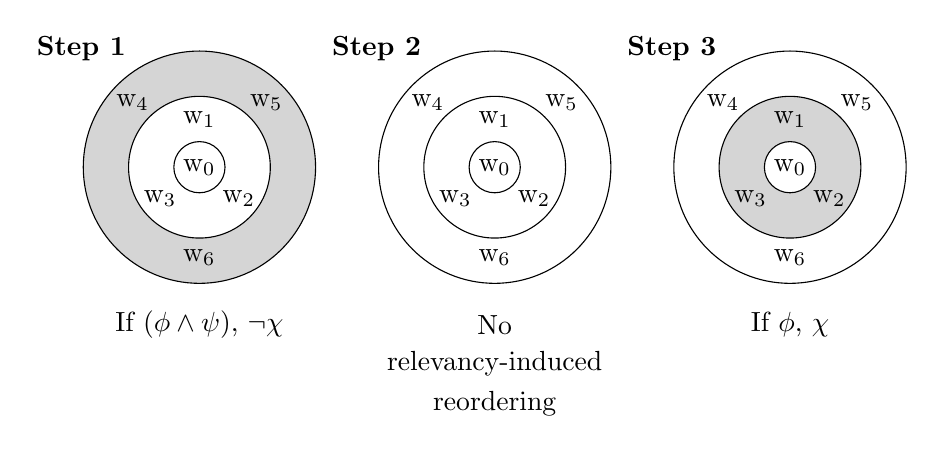
\begin{tikzpicture}
	\coordinate (O) at (0,0);
    \node at (-1.5,1.5) {\textbf{Step 1}};
	\draw[fill=gray!33] (O) circle (1.475);
	\draw[fill=white] (O) circle (0.9);
	\draw[fill=white] (O) circle (0.325)node {w$_0$};

	\node at (0,0.6) {w$_1$};
	\node at (0.5,-0.4) {w$_2$};
	\node at (-0.5,-0.4) {w$_3$};
	
	\node at (-0.85,0.825) {w$_4$};
	\node at (0.85,0.825) {w$_5$};
	\node at (0,-1.15) {w$_6$};
	
	\node at (0,-2) {If $(\phi\land\psi)$, $\neg\chi$};
	
	
	\begin{scope}[xshift=37.5mm]
		\coordinate (O) at (0,0);
        \node at (-1.5,1.5) {\textbf{Step 2}};
	\draw[fill=white] (O) circle (1.475);
	\draw[fill=white] (O) circle (0.9);
	\draw[fill=white] (O) circle (0.325)node {w$_0$};

	\node at (0,0.6) {w$_1$};
	\node at (0.5,-0.4) {w$_2$};
	\node at (-0.5,-0.4) {w$_3$};
	
	\node at (-0.85,0.825) {w$_4$};
	\node at (0.85,0.825) {w$_5$};
	\node at (0,-1.15) {w$_6$};
	
	\node at (0,-2) {No};
	\node at (0,-2.5) {relevancy-induced};
	\node at (0,-3) {reordering};
	
	\begin{scope}[xshift=37.5mm]
		\coordinate (O) at (0,0);
        \node at (-1.5,1.5) {\textbf{Step 3}};
	\draw[fill=white] (O) circle (1.475);
	\draw[fill=gray!33] (O) circle (0.9);
	\draw[fill=white] (O) circle (0.325)node {w$_0$};

	\node at (0,0.6) {w$_1$};
	\node at (0.5,-0.4) {w$_2$};
	\node at (-0.5,-0.4) {w$_3$};
	
	\node at (-0.85,0.825) {w$_4$};
	\node at (0.85,0.825) {w$_5$};
	\node at (0,-1.15) {w$_6$};
	
	\node at (0,-2) {If $\phi$, $\chi$};
	\end{scope}
	\end{scope}
\end{tikzpicture}
\caption{World orderings and selections of consistent reverse Sobel sequences according to \textcite{Lewis2018}. For all worlds $w_n$: If $n\geqslant1$, then $\phi=1$ is true for $w_n$, and if $n\geqslant 4$, then $\psi=1$ holds true for $w_n$.}
\labfig{lewis-heim-consistent}
\end{figure}
\noindent The instability concerning the felicity judgements of reverse Sobel sequences is also predicted by this account, as its sensitivity to discourse relevance grants the discourse participants some leeway in their semantic evaluation of the conditionals: \enquote{Hearing things at one moment as felicitous (consistent) and the next as infelicitous (inconsistent), or vice versa, is an expected feature of a phenomenon involving context sensitivity.} \parencite[p. 22]{Lewis2018}.

\subsection{Lewis (2018) and Causality}\labsec{lewis-klecha}
As noted by \textcite{Krassnig2017}, \textcite{Lewis2018} makes no distinction between acausal Sobel sequences and causal Sobel sequences. Whilst \citepos{Klecha2014} predictions were arguably too strong, as seen in \refsec{klecha-no}, his observation that reverse causal Sobel sequences are typically infelicitous still holds true. We therefore amend \citepos{Lewis2018} work to incorporate parts of \citepos{Klecha2014} analysis to make her account more viable. To do this, we start off with the same basic assumption that was required by Klecha's analysis: \textcite{Bennett2003} and \citepos{Arregui2009} view on world ordering. The incorporation of their work into Lewis' framework has only one currently relevant impact: The similarity ordering of causal Sobel sequences is such that $\phi$-worlds and $\phi\land\psi$-worlds are equally similar to the evaluation world. Contrary to Klecha's model, this poses no immediate issue, since similarity is no longer the sole determining factor for world closeness. Assuming that low relevance pulls these $\phi\land\psi$-worlds further away from the evaluation world, these worlds would no longer be counted amongst the closest $\phi$-worlds for the evaluation of the $\phi$-conditional in a causal Sobel sequence. This assumption of low relevance is common in the literature: \textcite{Moss2012}, \textcite{Klecha2014,Klecha2015}, and \textcite{Lewis2018} all make the same (implicit or explicit) assumption in one way or another. Klecha, in particular, requires the implicit assumption that $\phi\land\psi$-worlds are contextually less relevant than the $\phi$-worlds to motivate the low level of precision a causal Sobel sequence starts out with.\footnote{Lewis actually states that low precision is comparable to lower relevance in her framework \parencite[p. 500]{Lewis2018}, though she does not correlate this to (reverse) Sobel sequences.} Lewis, on the other hand, explicitly states that certain possibilities can be considered contextually irrelevant for discourse purposes (i.e. the speaker trying to make a point) until some discourse participants brings them into play \parencite[p. 501]{Lewis2018}. Whilst she was talking about Sobel sequences in general, it certainly fits the description of what appears to be happening to causal Sobel sequences. Once these worlds are pulled further away from the evaluation world by their contextual irrelevance, the remaining evaluation of the sequence is true to the standard variably-strict analysis, as is seen in figure~\reffig{hybrid-lewis}.%
\begin{figure}[!htb]
\begin{tikzpicture}
	\coordinate (O) at (0,0);
	\node at (-1.5,1.5) {\textbf{Step 1}};
		\draw[fill=white] (O) circle (1.475);
		\draw[fill=white] (O) circle (0.9);
		\draw[fill=white] (O) circle (0.325)node {w$_0$};
	
	\node at (0,0.6) {w$_1$};
	\node at (0.5,-0.4) {w$_2$};
	\node at (-0.5,-0.4) {w$_3$};
	
	\node at (-0.5,0.4) {w$_4$};
	\node at (0.5,0.4) {w$_5$};
	\node at (0.025,-0.6) {w$_6$};
	
	\node at (0.2,-2) {Relevancy-induced};
	\node at (0.2,-2.5) {reordering};
	
		
		\draw[color=black!75,line width=0.5mm,>={Triangle[length=2mm,width=2mm]},->] (0.7,0.7) --(1,1);
		\draw[color=black!75,line width=0.5mm,>={Triangle[length=2mm,width=2mm]},->] (-0.7,0.7) -- (-1,1);
		\draw[color=black!75,line width=0.5mm,>={Triangle[length=2mm,width=2mm]},->] (0,-1) -- (0,-1.4);
	
	\begin{scope}[xshift=37.5mm]
		\coordinate (O) at (0,0);
	    \node at (-1.5,1.5) {\textbf{Step 2}};
		\draw[fill=white] (O) circle (1.475);
		\draw[fill=gray!33] (O) circle (0.9);
		\draw[fill=white] (O) circle (0.325)node {w$_0$};
	
	\node at (0,0.6) {w$_1$};
	\node at (0.5,-0.4) {w$_2$};
	\node at (-0.5,-0.4) {w$_3$};
	
	\node at (-0.85,0.825) {w$_4$};
	\node at (0.85,0.825) {w$_5$};
	\node at (0,-1.15) {w$_6$};
	
		\node at (0,-2) {If $\phi$, $\chi$};
	
	
	\begin{scope}[xshift=37.5mm]
		\coordinate (O) at (0,0);
        \node at (-1.5,1.5) {\textbf{Step 3}};
	\draw[fill=gray!33] (O) circle (1.475);
	\draw[fill=white] (O) circle (0.9);
	\draw[fill=white] (O) circle (0.325)node {w$_0$};

	\node at (0,0.6) {w$_1$};
	\node at (0.5,-0.4) {w$_2$};
	\node at (-0.5,-0.4) {w$_3$};
	
	\node at (-0.85,0.825) {w$_4$};
	\node at (0.85,0.825) {w$_5$};
	\node at (0,-1.15) {w$_6$};
	
	\node at (0,-2) {If $(\phi\land\psi)$, $\neg\chi$};
	\end{scope}
	\end{scope}
\end{tikzpicture}
\caption{Proposed world closeness orderings and domains of causal Sobel sequences. For all worlds $w_n$: If $n\geqslant1$, then $\phi=1$ is true for $w_n$, and if $n\geqslant 4$, then $\psi=1$ holds true for $w_n$.}
\labfig{hybrid-lewis}
\end{figure}
In this, causal Sobel sequences differ from the analysis of acausal Sobel sequences: In order to make the $\phi$-conditional a true statement, causal Sobel sequences require low relevance to interfere with the similarity ordering, whereas acausal Sobel sequences require nothing of the sort.

Having demonstrated that causal Sobel sequences pose no immediate problem, we turn to their reverse counterparts. There are two ways a reverse causal Sobel sequence can be judged as infelicitous: A pure reverse causal Sobel sequence requires no special steps. The initial discourse context acknowledges the relevance of the $\phi\land\psi$-worlds and thereby does not pull them further away from the evaluation world. The $\phi$-conditional also ranges over the $\phi\land\psi$-worlds, leading to a contradictory statement. A more interesting case is the reverse causal Sobel sequence in \refex{klecha2}, repeated below as \refex{klecha2-repeat2}, where the reverse causal Sobel sequence is embedded within a standard causal Sobel sequence. 
\pex\phantomsection\labex{klecha2-repeat2}%
\contextpex{Construction workers Daryl, Aaron, and Ida, stand around a construction site.  Daryl is not wearing a helmet.  A large beam falls from above them and lands where no one was standing, but near to Daryl.}
			\a	\speaker{Aaron}Daryl, if you had been standing there, you would have been killed.
			\a	\speaker{Ida}But if he had been standing there and he saw the shadow of the falling beam and managed to jump out of the way in time, he would not have.
			\a	\speaker{Aaron}\#Exactly. But what I said is still right:  If you had been
standing there, you would have been killed.\hfill\parencite[adapted from][p. 153f]{Klecha2014}
\xe
Since the $\phi\land\psi$-worlds were originally moved further away from the evaluation world, they need to be pulled back in, in order to make the reverse causal Sobel sequence inconsistent. Whether or not the $\phi\land\psi$-worlds are counted amongst the closest $\phi$-worlds is then dependent upon the same criteria previously posited: 
\begin{enumerate}
    \item The possibility of $\phi\land\psi$ needs to be salient
    \item The closest $\phi$-worlds and $\phi\land\psi$-words need to be similar enough to one another
    \item $\phi\land\psi$ needs to be relevant to the current discourse 
\end{enumerate}
The first criteria is automatically fulfilled, as the possibility of an antecedent is always raised to salience. The second criteria is also automatically fulfilled, since $\phi\land\psi$-worlds and $\phi$-worlds are equally similar in causal Sobel sequences. Therefore, the sole deciding factor for causal Sobel sequences is the relevance to the current discourse. This criteria is also, in most cases, automatically fulfilled: We would argue that any question under discussion that considers it relevant whether or not $\chi$ would follow from $\phi$ would also be sensitive to any possibility $\psi$ that is directly or indirectly caused by $\phi$ and that could possibly prevent $\chi$ from happening.

Positing all of Lewis' criteria would also predict, however, that the worlds in question must not be intrinsically irrelevant: They must be considered at least realistic, even if highly improbable, by the discourse participants. We would therefore predict that some reverse causal Sobel sequences are consistent, even if no explicit questioning of the relevance of $\phi\land\psi$-worlds takes place (as was indirectly done in \refex{rLS-felicitous-psi2}). This prediction appears to hold true, considering the reverse causal Sobel sequence in \refex{quantum}.
\ex\phantomsection\labex{quantum}\textit{Speaker A transported a vase between two points, in a barren stone room lacking any soft surfaces that might cushion a potential fall of the vase.}\\
\ljudge{A: }If I had dropped that vase, it would have broken.\\
\ljudge{B: }But if you had dropped that vase and that drop caused it to quantum-tunnel to a cushy pillow, it would not have.\\
\ljudge{A: }Okay, but what I said is still true: If I had dropped it, it would have broken.
\xe

Finally, we need to account for the felicitous reverse causal Sobel sequence in \refex{rLS-felicitous}, repeated below as \refex{rLS-felicitous-repeat}, where the relevance of the $\phi\land\psi$-worlds was overtly denigrated. 
\pex\phantomsection\labex{rLS-felicitous-repeat}%
\contextpex{Construction workers Daryl, Aaron, and Ida, stand around a construction site.  Daryl is not wearing a helmet.  A large beam falls from above them and lands where no one was standing, but near to Daryl. Daryl is also known to possess exceptionally bad reflexes: Generally, nine out of ten attempts to evade something as fast as the falling steel beam result in failure.}
	\a\phantomsection\labex{rLS-felicitous-phi-repeat}\speaker{Aaron}Daryl, if you had been standing there, you would have been killed.
	\a\phantomsection\labex{rLS-felicitous-phipsi-repeat}\speaker{Ida}But if he had been standing there and he saw the shadow of the falling beam and managed to jump out of the way in time, he would not have.
	\a\phantomsection\labex{rLS-felicitous-psi2-repeat}\speaker{Aaron}Sure, that may be possible, but the chances of that happening are like really, really low. So, my point stands: If he had stood there, he would have died.\hfill\parencite[adapted and modified from][p. 134]{Klecha2014}
\xe
Here, the explanation of its felicity is simplistically straightforward within \citepos{Lewis2018} amended framework. The probability of the $\phi\land\psi$-worlds are explicitly asserted to be highly improbable. In most cases, probability and relevance are almost intrinsically tied together.  By questioning their probability, the speaker also implicitly questioned their relevance to the discourse. In doing so, the discourse participant pushes the $\phi\land\psi$-worlds further away from the evaluation world, again, which leaves them free to reassert their original conditional without inconsistency. 

This is visually represented in \reffig{hybrid-relevance-retract}.
\noindent\begin{figure}[!htb]
\resizebox{!}{92mm}{\begin{tikzpicture}
	\coordinate (O) at (0,0);
	\node at (-1.5,1.5) {\textbf{Step 1}};
		\draw[fill=white] (O) circle (1.475);
		\draw[fill=white] (O) circle (0.9);
		\draw[fill=white] (O) circle (0.325)node {w$_0$};
	
		\node at (0,0.6) {w$_1$};
		\node at (0.5,-0.4) {w$_2$};
		\node at (-0.5,-0.4) {w$_3$};
	
		\node at (0.025,-0.6) {w$_6$};
		\node at (-0.5,0.4) {w$_4$};
		\node at (0.5,0.4) {w$_5$};
	
		\node at (0,-2) {Relevancy};
		\node at (0,-2.5) {reordering};
		
		\draw[color=black!75,line width=0.5mm,>={Triangle[length=2mm,width=2mm]},->] (0.7,0.7) --(1,1);
		\draw[color=black!75,line width=0.5mm,>={Triangle[length=2mm,width=2mm]},->] (-0.7,0.7) -- (-1,1);
		\draw[color=black!75,line width=0.5mm,>={Triangle[length=2mm,width=2mm]},->] (0,-1) -- (0,-1.4);
		
	
	\begin{scope}[xshift=37.5mm]
		\coordinate (O) at (0,0);
		\node at (-1.5,1.5) {\textbf{Step 2}};
	
		\draw[fill=white] (O) circle (1.475);
		\draw[fill=gray!33] (O) circle (0.9);
		\draw[fill=white] (O) circle (0.325)node {w$_0$};
	
		\node at (0,0.6) {w$_1$};
		\node at (0.5,-0.4) {w$_2$};
		\node at (-0.5,-0.4) {w$_3$};
	
	\node at (0,-1.2) {w$_6$};
	\node at (-0.85,0.8) {w$_4$};
	\node at (0.85,0.8) {w$_5$};
	
		\node at (0,-2) {If $\phi$, $\chi$};
	
	
	\begin{scope}[xshift=37.5mm]
		\coordinate (O) at (0,0);
\node at (-1.5,1.5) {\textbf{Step 3}};
	\draw[fill=gray!33] (O) circle (1.475);
	\draw[fill=white] (O) circle (0.9);
	\draw[fill=white] (O) circle (0.325)node {w$_0$};

	\node at (0,0.6) {w$_1$};
	\node at (0.5,-0.4) {w$_2$};
	\node at (-0.5,-0.4) {w$_3$};
	
	\node at (0,-1.2) {w$_6$};
	\node at (-0.85,0.8) {w$_4$};
	\node at (0.85,0.8) {w$_5$};
	
	\node at (0,-2) {If $(\phi\land\psi)$, $\neg\chi$};

	
	\begin{scope}[yshift=-47.5mm,xshift=-75mm]
		\coordinate (O) at (0,0);
	\node at (-1.5,1.5) {\textbf{Step 4}};
		\draw[fill=white] (O) circle (1.475);
		\draw[fill=white] (O) circle (0.9);
		\draw[fill=white] (O) circle (0.325)node {w$_0$};
	
		\node at (0,0.6) {w$_1$};
		\node at (0.5,-0.4) {w$_2$};
		\node at (-0.5,-0.4) {w$_3$};
	
		\node at (0.025,-0.6) {w$_6$};
		\node at (-0.5,0.4) {w$_4$};
		\node at (0.5,0.4) {w$_5$};
	
		\node at (0,-2) {Proposed};
		\node at (0,-2.5) {reordering};
		
		\draw[color=black!75,line width=0.5mm,>={Triangle[length=2mm,width=2mm]},<-] (0.7,0.7) --(1,1);
		\draw[color=black!75,line width=0.5mm,>={Triangle[length=2mm,width=2mm]},<-] (-0.7,0.7) -- (-1,1);
		\draw[color=black!75,line width=0.5mm,>={Triangle[length=2mm,width=2mm]},<-] (0,-1) -- (0,-1.4);
		
		
		\begin{scope}[xshift=37.5mm]
		\coordinate (O) at (0,0);
	\node at (-1.5,1.5) {\textbf{Step 5}};
		\draw[fill=white] (O) circle (1.475);
		\draw[fill=white] (O) circle (0.9);
		\draw[fill=white] (O) circle (0.325)node {w$_0$};
	
		\node at (0,0.6) {w$_1$};
		\node at (0.5,-0.4) {w$_2$};
		\node at (-0.5,-0.4) {w$_3$};
	
		\node at (0.025,-0.6) {w$_6$};
		\node at (-0.5,0.4) {w$_4$};
		\node at (0.5,0.4) {w$_5$};
	
		\node at (0,-2) {Denigration of};
		\node at (0,-2.5) {relevance of};
		\node at (0,-3) {$\phi\land\psi$-worlds};
		
		\draw[color=black!75,line width=0.5mm,>={Triangle[length=2mm,width=2mm]},->] (0.7,0.7) --(1,1);
		\draw[color=black!75,line width=0.5mm,>={Triangle[length=2mm,width=2mm]},->] (-0.7,0.7) -- (-1,1);
		\draw[color=black!75,line width=0.5mm,>={Triangle[length=2mm,width=2mm]},->] (0,-1) -- (0,-1.4);
		
		
		\begin{scope}[xshift=37.5mm]
		\coordinate (O) at (0,0);
	\node at (-1.5,1.5) {\textbf{Step 6}};
		\draw[fill=white] (O) circle (1.475);
		\draw[fill=gray!33] (O) circle (0.9);
		\draw[fill=white] (O) circle (0.325)node {w$_0$};
	
		\node at (0,0.6) {w$_1$};
		\node at (0.5,-0.4) {w$_2$};
		\node at (-0.5,-0.4) {w$_3$};
	
	\node at (0,-1.2) {w$_6$};
	\node at (-0.85,0.8) {w$_4$};
	\node at (0.85,0.8) {w$_5$};
	
		\node at (0,-2) {If $\phi$, $\chi$};
		\end{scope}
	\end{scope}
	\end{scope}
	\end{scope}
	\end{scope}
\end{tikzpicture}}
\caption{Proposed world closeness orderings and world selections of \refex{rLS-felicitous}. For all worlds $w_n$: If $n\geqslant1$, then $\phi=1$ is true for $w_n$, and if $n\geqslant 4$, then $\psi=1$ holds true for $w_n$.}
\labfig{hybrid-relevance-retract}
\end{figure}
There, Step 1 presents the discourse-initial effect of relevance upon the world closeness ordering, rendering the worlds $w_4$, $w_5$, and $w_6$ less close than similar to the evaluation world $w_0$ via context. The $\phi$-conditional in \refex{rLS-felicitous-phi-repeat} is then evaluated based upon this world closeness ordering in Step 2, which does not further affect the world closeness ordering. This is followed by the evaluation of the $\phi\land\psi$-conditional in \refex{rLS-felicitous-phipsi-repeat} in Step 3, which subsequently affects the world closeness ordering. Step 4 presents the proposed shift in world closeness due to the salience-based increase in relevance of the $\phi\land\psi$-worlds. In Step 5, the overt denigration of these worlds' relevance in \refex{rLS-felicitous-psi2-repeat} undoes this process by pushing them further away from the evaluation world again. This leads to Step 6, where the $\phi$-conditional is felicitously re-asserted in \refex{rLS-felicitous-psi2-repeat}.


\textcite{Lewis2018}, as amended by us in this section to account for causal Sobel sequences, would therefore leave us with the following predictions concerning the felicity of reverse Sobel sequences in \reftab{Lewis-amended}:
\begin{table}[!htb]
\caption{Predictions of \textcite{Lewis2018}, incorporating \textcite{Bennett2003} or \textcite{Arregui2009}, to distinguish between acausal Sobel sequences and causal Sobel sequences.}\resizebox{\textwidth}{!}{%
    \begin{tabular}{lcccc}
    \toprule
                &   \multicolumn{2}{c}{Causally Unrelated}    &   \multicolumn{2}{c}{Causally Related}\\
                &   Similar Worlds  &   Dissimilar Worlds   & Non-Denigrated    & Denigrated  \\\midrule
          Regular Order &   \checkmark  &   \checkmark  &   \checkmark  &   \checkmark\\
          Reverse Order &   \#  &   \checkmark          &   \#  &   \checkmark\\
          \bottomrule
    \end{tabular}}\labtab{Lewis-amended}
\end{table}

Taking stock, to account for the (in-)felicity of reverse Sobel sequences, we currently require the following ingredients: (i) the (a)causal relation between antecedent propositions \parencite{Klecha2014,Klecha2015}, (ii) contrastive stress \parencite{Klecha2014,Klecha2015}, and (iii) relevance affecting which worlds are quantified over \parencite{Lewis2018}. Whilst it is evident that relevance is a critical factor in correctly predicting reverse Sobel sequence (in-)felicity, as shown in \refex{rLS-felicitous}=\refex{rLS-felicitous-repeat} and \refex{quantum}, it is not clear to us whether the way it was formally implemented by \textcite{Lewis2018} in its interaction with world similarity is necessarily correct. We further motivate and explore these doubts in \refsec{experiment}.

\section{Experimental Testing of Lewis (2018)}\labsec{experiment}
With \reftab{Lewis-amended}, we have a function-like prediction distribution that is not strictly contradicted by the empirical data presented up until this point. This is partially due to the nature of its factors: It proved far more difficult to receive clear-cut acceptability judgements by native speakers via informal methods when it comes to dissimilar reverse Sobel sequences and similar reverse Sobel sequences than with any of the previously tested factors. As such, in \textcite{Krassnig2020}, we decided to conduct an experiment  (i) to finally bring some experimental data into the discussion of reverse Sobel sequences, and (ii) to test the predictions made by \textcite{Lewis2018}. To avoid further complicating the experiment, we decided against testing for \citepos{Klecha2014,Klecha2015} predictions regarding the effect of causality upon reverse Sobel sequence felicity, as they were already nigh universally confirmed by the native speakers we consulted---contrary to the feedback we received regarding varying degrees of dissimilarity.
\subsection{Material \& Methods}\labsec{materialmethods}
To accomplish our two goals, testing Lewis' hypothesis concerning the effect of world similarity on infelicity and testing whether or not disjoint antecedent worlds reverse Sobel sequences are as acceptable as regular sentences, we have formulated two hypotheses which shaped our experiment's design: 
\begin{enumerate}
    \item If two reverse Sobel sequences are the same except for the degree of similarity between their conditionals' antecedent worlds, then the reverse Sobel sequence whose degree of similarity is more disparate should be considered more acceptable on average. (hereafter the \textit{dissimilar worlds hypothesis})
    \item If the domains of quantification of a reverse Sobel sequence are entirely disjoint, there should be no difference in acceptability between them and regular sentences (i.e. the control items). (hereafter the \textit{disjoint domain hypothesis})
\end{enumerate}
The disjoint domain hypothesis serves two purposes: (i) It tests whether reverse Sobel sequences are ever as felicitous as non-reverse Sobel sequences, and (ii), more crucially, the results gathered from testing this hypothesis act as a positive baseline to compare the results of the dissimilar worlds hypothesis against.

\subsubsection{Materials}\labsec{materials}
In order to test the dissimilar worlds hypothesis, we created five experimental items which contain a reverse Sobel sequence each and were presented with two different contexts: Differing as little as possible, they either indicate that the $\phi\land\psi$-worlds and $\phi$-worlds are very similar to one another or very dissimilar to one another. These respectively represent the {\scshape similar} and {\scshape dissimilar} conditions. From a syntactic point of view, all conditionals are future-less-vivids and, deviating from the classical examples, contain the auxiliary verb \textit{did} in front of the $\phi$-antecedent's main verb. The auxiliary verb was inserted in order to ensure that the $\phi$-conditional's antecedent is not a syntactic subset of the $\phi\land\psi$-conditional's antecedent. This was necessary, since \textcite[p. 135]{Klecha2015} posited that the $\phi$-antecedent being a syntactic subset of the previous conditional's antecedent would automatically render the reverse Sobel sequence infelicitous, as some form of contrastive stress in the second conditional is required. The attentive reader may have noticed that we already encountered a counterexample to this restriction in \refex{match}=\refex{match-repeat}, repeated again below as \refex{match-repeat2}. 
\ex\phantomsection\labex{match-repeat2}\context{Holding up a dry match, with no water around.}If I had struck this match and it had been soaked, it would not have lit. But if I \MakeUppercase{had} struck this match, it would have lit.\\%
\emptyfill(adapted from \textcite[p. 106]{Stalnaker1968} by \textcite[p. 487]{Lewis2018})
\xe
However, preliminary testing with native speakers of English ($n=12$) prior to the experiment has shown (i) that the auxiliary verb \textit{had} appears obligatorily stressed in this reverse Sobel sequence, even though it is present in either of the sequence's conditionals, and that (ii) this reverse Sobel sequence is rendered less acceptable by turning it into the future-less-vivid conditional in \refex{match-flv}. 
\ex\phantomsection\context{Holding up a dry match, with no water around.}If I struck this match and it was soaked, it would not light. ?But if I struck this match, it would light.\labex{match-flv}
\xe
Introducing either \textit{did} or \textit{were to} then improved the acceptability for the same native speakers of English, as seen in \refex{match-flv-did} and \refex{match-flv-were}, respectively.\\
\begin{minipage}{\linewidth}\pex\phantomsection\contextpex{Holding up a dry match, with no water around.}
\a\phantomsection\phantomsection If I struck this match and it was soaked, it would not light. But if I \MakeUppercase{did} strike this match, it would light.\labex{match-flv-did}
\a\phantomsection\phantomsection If I struck this match and it was soaked, it would not light. But if I \MakeUppercase{were} to strike this match, it would light.\labex{match-flv-were}
\xe\end{minipage}
As the consulted native speakers unanimously agreed with this observation, we decided not to experimentally verify this and decided on using \textit{did} for the sake of simplicity in our experiment. For more on the necessity of contrastive stress and its placement on the auxiliary verb, we refer to \refsec{introspection}.

    
In total, this led us to the experimental pattern in \refdef{pattern-lewis}, which, in turn, led us to our experimental items, as seen in \refex{pattern-lewis}. The remainder of the experimental target items may be found in \refapp{items}.
\ex\phantomsection \context{Context text common to either condition combined with \ldots \\
    \ljudge{(i) } \ldots text that sets the $\phi\land\psi$-worlds and $\phi$-worlds as similar to one another.\\
    \ljudge{(ii) } \ldots text that sets the $\phi\land\psi$-worlds and $\phi$-worlds as dissimilar to one another.}
    \speaker{S}If $\phi\land\psi$, (then) $\neg\chi$; but if did-$\phi$, (then) $\chi$.\labdef{pattern-lewis}
\xe
\ex\phantomsection\context{Andy's friend Michael plans to go to a cabin in the woods during the semester break. He is not convinced, however, that it will be a fun trip, because he is terrified of storms and he would have no way out if one took place.\\
    \ljudge{(i) } His trip would be during an average month of the year and Andy thinks that a storm would be possible but not too likely.\\
    \ljudge{(ii) } His trip would be during the driest month of the year and Andy thinks that a storm would be impossible or at the very least extremely unlikely.}
    \speaker{Andy}If you went to the cabin and a storm came, your trip would be horrible; but if you \MakeUppercase{did} go to the cabin, it would be a pretty good trip.\labex{pattern-lewis}
\xe

In order to test the disjoint domain hypothesis, we furthermore created five experimental items that also contain a reverse Sobel sequence each, but which were presented with only one context. These represent the {\scshape disjoint} condition. Aside from the context, and a subsequent sentence explicating the purpose of the reverse Sobel sequence, these items are identical in shape to the previously shown experimental items. However, there is one difference which pertains to the hypothesis tested: Whilst the $\phi$-conditional remains a standard future-less-vivid conditional, the $\phi\land\psi$-conditional concerns itself with an epistemically excluded possibility because $\psi$ is either contrary to fact or has been excluded as a possibility by the speaker, though it retains the same overt tense structure as the other conditionals. This shift from epistemically excluded to live possibilities is motivated by the fact that both variably-strict and (semi-)dynamic strict conditional models would generally assume that conditionals about live possibilities would not take epistemically excluded worlds into account. As such, either approach should predict felicity. See \refex{Klecha} for an example item. The remaining experimental target items may be found in \refapp{items}.
\ex\phantomsection\context{Alex and her friend Steve enter a construction site. Steve doesn't wear his helmet, but carries it around in his hand. This annoys Alex, since it's a dangerous site.}
\speaker{Alex}If some construction material fell on your head right now and you wore a helmet, you would probably survive the incident; but if some construction material \MakeUppercase{did} fall on your head right now, you would certainly die. So, wear your goddamn helmet.\labex{Klecha}
\xe

We also created 20 control items, representing the {\scshape control} condition, that acted as fillers. These consisted of non-reverse Sobel sequences, generic conditional sequences, and reverse Sobel sequence containing an exhaustifying lexical item (e.g. \textit{only}). These items were also displayed with an appropriate context.

The total number of conditions were distributed across three lists in a Latin square design, as shown in \reftab{list}. 
\begin{table}[!htb]
    \caption{Latin square condition lists assigned to participants, the condition {\scshape similar} represented as A, {\scshape dissimilar} as B, and {\scshape disjoint} as C.}
    \label{list-nofillers}
    \begin{tabular}{ll}\toprule
        List & Item Order\\\midrule
        I & A B C A B C A B C A B C A B C\\
        II & B A B C A B C A B C A B C A B\\
        III & A C A B C A B C A B C A B C A\\
        \bottomrule
    \end{tabular}\labtab{list}
\end{table}
The fillers, i.e. control items, were then added to these lists such that no target condition is directly followed by another target condition, yielding the final lists shown in \reftab{list-full}.
\begin{table}[!htb]
    \caption{Latin square condition lists assigned to participants, target conditions in boldface and fillers represented as {\scshape f}, the {\scshape similar} condition as A, {\scshape dissimilar} as B, and {\scshape disjoint} as C.}
    \labtab{list-full}
    \resizebox{\textwidth}{!}{%
    \begin{tabular}{ll}\toprule
    List & Item order\\\midrule
        I & {\scshape {\scshape f}} \textbf{A} {\scshape f} \textbf{B} {\scshape f} {\scshape f} \textbf{C} {\scshape f} \textbf{A} {\scshape f} \textbf{B} {\scshape f} \textbf{C} {\scshape f} \textbf{A} {\scshape f} {\scshape f} \textbf{B} {\scshape f} \textbf{C} {\scshape f} \textbf{A} {\scshape f} \textbf{B} {\scshape f} \textbf{C} {\scshape f} {\scshape f} \textbf{A} {\scshape f} \textbf{B} {\scshape f} {\scshape f} \textbf{C} {\scshape f}\\
        II & {\scshape f} \textbf{C} {\scshape f} \textbf{A} {\scshape f} {\scshape f} \textbf{B} {\scshape f} \textbf{C} {\scshape f} \textbf{A} {\scshape f} \textbf{B} {\scshape f} \textbf{C} {\scshape f} {\scshape f} \textbf{A} {\scshape f} \textbf{B} {\scshape f} \textbf{C} {\scshape f} \textbf{A} {\scshape f} \textbf{B} {\scshape f} {\scshape f} \textbf{C} {\scshape f} \textbf{A} {\scshape f} {\scshape f} \textbf{B} {\scshape f}\\
        III & {\scshape f} \textbf{B} {\scshape f} \textbf{C} {\scshape f} {\scshape f} \textbf{A} {\scshape f} \textbf{B} {\scshape f} \textbf{C} {\scshape f} \textbf{A} {\scshape f} \textbf{B} {\scshape f} {\scshape f} \textbf{C} {\scshape f} \textbf{A} {\scshape f} \textbf{B} {\scshape f} \textbf{C} {\scshape f} \textbf{A} {\scshape f} {\scshape f} \textbf{B} {\scshape f} \textbf{C} {\scshape f} {\scshape f} \textbf{A} {\scshape f}\\\bottomrule
    \end{tabular}
    }\labtab{listfiller}
\end{table}


Each participant was randomly assigned to one of the three item lists. Concerning the actual test items themselves, these were also randomly assigned for each participant to each pre-placed condition slot in the randomly assigned item list, whilst the fillers were fixed in place across all lists. As such, each participant had a partially randomised item list specific to them.

There were a total of 48 participants, of which 41 remained after all exclusions. The criteria for exclusion are elaborated upon in \refsec{method}.


\subsubsection{Methods}\labsec{method}
The experiment itself was an acceptability rating study. Prior to participating in the study, the participants were asked to provide information concerning their age, gender, native language, whether they were raised bilingually, and other languages spoken. They were then asked to sign an agreement, that their anonymised data may be used, statistically processed, and published in its processed, anonymised form. This was followed by an explanation of what they had to do.

The participants were then individually shown and asked to rate the acceptability of each test items on a Likert scale from 1 (=\textit{sounds very natural}) to 5 (=\textit{sounds very unnatural}). Upon having rated a test item, the participants had to click a button to continue to the next item. The participants were unable to go back and re-rate an earlier test item.

Participants were excluded if they (i) failed to rate 75\% of all control items three or better, (ii) provided an age below 18 or above 65, %
(ii) were either non-native speakers of English or were raised bilingually, or (iv) did not complete the entire experiment run.

The experiment was conducted entirely online, and the participants were gathered from various social network sites. Participation was entirely voluntary and not financially compensated.

\subsection{Results}\labsec{results}
From the results, it was clear that the control items were rated the most acceptable, followed by the {\scshape disjoint} reverse Sobel sequence, the {\scshape dissimilar} reverse Sobel sequence, and finally by the {\scshape similar} reverse Sobel sequence: 
\begin{table}[!htb]
    \caption{Average acceptability of each condition, ranked from highest to lowest}
    \labtab{average-results}
    \begin{tabular}{lrr}
    \toprule
        Condition & Average Acceptability & Variance\\\midrule
        {\scshape control} Condition & 1.48 & 0.45 \\
        {\scshape disjoint} Condition & 2.15 & 0.65 \\
        {\scshape dissimilar} Condition & 3.41 & 1.54 \\
        {\scshape similar} Condition & 4.4 & 0.43\\
        \bottomrule
    \end{tabular}
\end{table}

We analysed the obtained data with a one-factor ANOVA, which showed a statistically significant difference between groups as determined by one-way ANOVA ($F(3,1021) = 643.1$, $p < .01$). Post hoc conducted one-tailed t-tests between each condition showed that there is a significant difference between each condition: Comparing the {\scshape control} condition to the {\scshape disjoint} condition, we obtained $t(204)=-8.8, p<0.05$, to the {\scshape dissimilar} condition, $t(204)=-19.3, p<0.05$, and to the {\scshape similar} condition, $t(204)=-45.1, p<0.05$. Comparing the {\scshape similar} condition to the {\scshape dissimilar} condition, we obtain $t(204)=10.3, p<0.05$, and to the {\scshape disjoint} condition, $t(204)=30.7, p<0.05$. Comparing the {\scshape dissimilar} condition to the {\scshape disjoint} condition, we obtain $t(204)=12.2, p<0.05$.

The comparatively high variance of the {\scshape dissimilar} condition led us to take a closer look at its raw data: Intuitively, it seemed that some participants consistently rated these items far lower than other participants. We therefore opted to test our intuition with a k-means clustering analysis, to see if our participants could be divided into more than one population. The cluster analysis of the participants' results showed that the data could be split into two distinct populations, with relatively high values of confidence. The first population cluster, Cluster 1, consists of 26 participants (i.e. 63\% of all participants), and the second population cluster, Cluster 2, consists of 15 participants (i.e. 37\% of all participants).
\begin{figure}[!htb]
    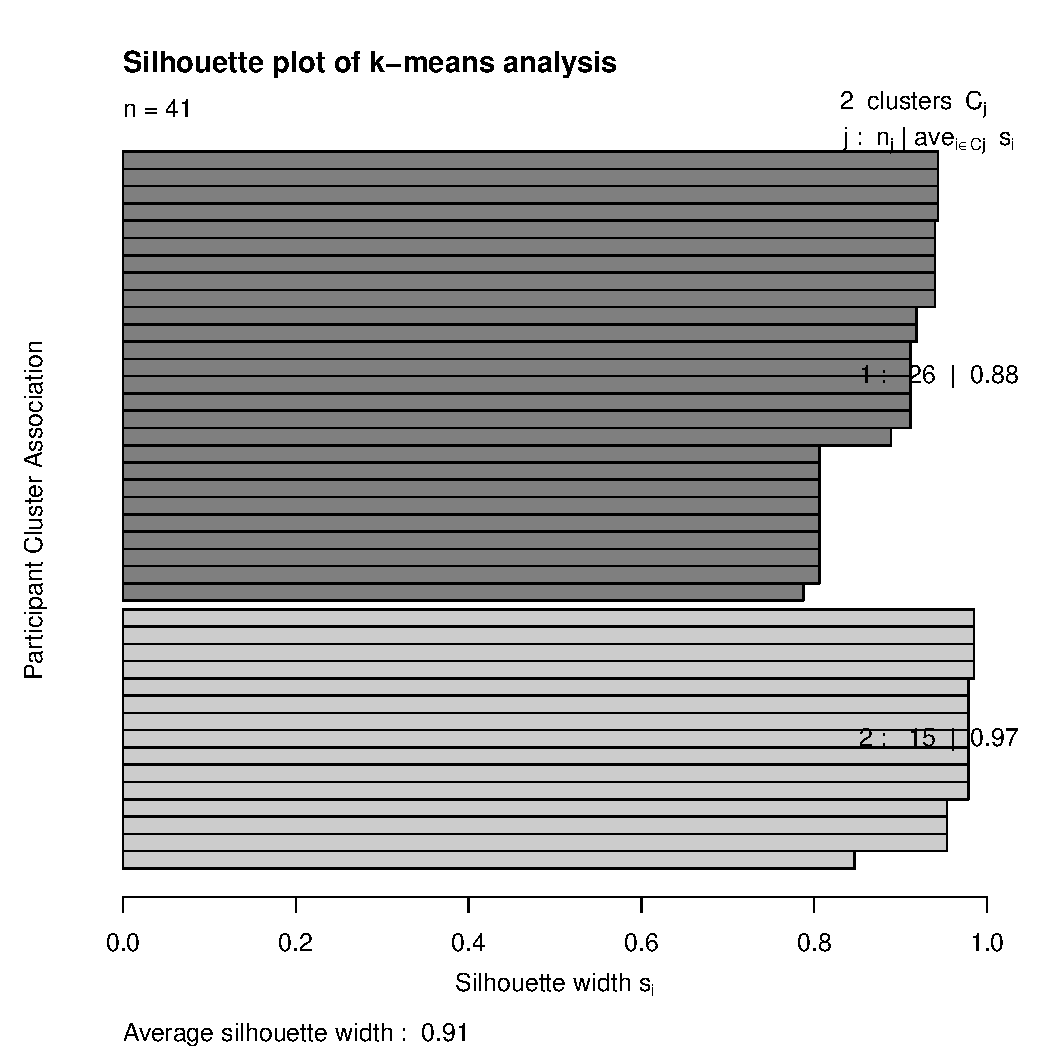
\includegraphics[width=0.69\linewidth]{silhouette.pdf}
    \caption{Silhouette plot of k-means analysis of participants by acceptability ratings}
    \labfig{silhouette plot}
\end{figure}

Subsequent one-tailed t-tests showed that there are no differences for each condition between population clusters except for the {\scshape dissimilar} condition with $t(69)=10.5, p<0.05$. For the {\scshape control} condition, we obtain $t(139)=-0.6, p>0.1$, for the {\scshape similar} condition, $t(69)=0.7, p>0.1$, and for the {\scshape disjoint} condition, $t(69)=0.3, p>0.1$.

For the {\scshape dissimilar} condition, the variance and acceptability is greatly reduced for Cluster 2, as shown in \reftab{average-results-pops} and \reffig{boxplot}:
\begin{table}[!htb]
    \caption{Average acceptability of each condition, divided by population cluster}
    \labtab{average-results-pops}
    \begin{tabular}{lrrrr}
    \toprule
        Condition & \multicolumn{2}{r}{Average Acceptability} & \multicolumn{2}{r}{Variance}\\\midrule
                        & Cluster 1       & Cluster 2       & Cluster 1 & Cluster 2\\\cmidrule[0.1pt](lr{0.1em}){2-3}\cmidrule[0.1pt](lr{0.1em}){4-5}
        {\scshape control}    & 1.50  & 1.44&   0.47      &  0.41\\
        {\scshape disjoint}   & 2.13  & 2.17 &   0.65     &  0.67\\
        {\scshape dissimilar} & 2.87  & 4.46 &   1.21     &  0.51\\
        {\scshape similar}    & 4.38  &   4.44  & 0.45  &  0.40\\
        \bottomrule
    \end{tabular}
\end{table}
\begin{figure}[!htb]
\begin{minipage}{\linewidth}
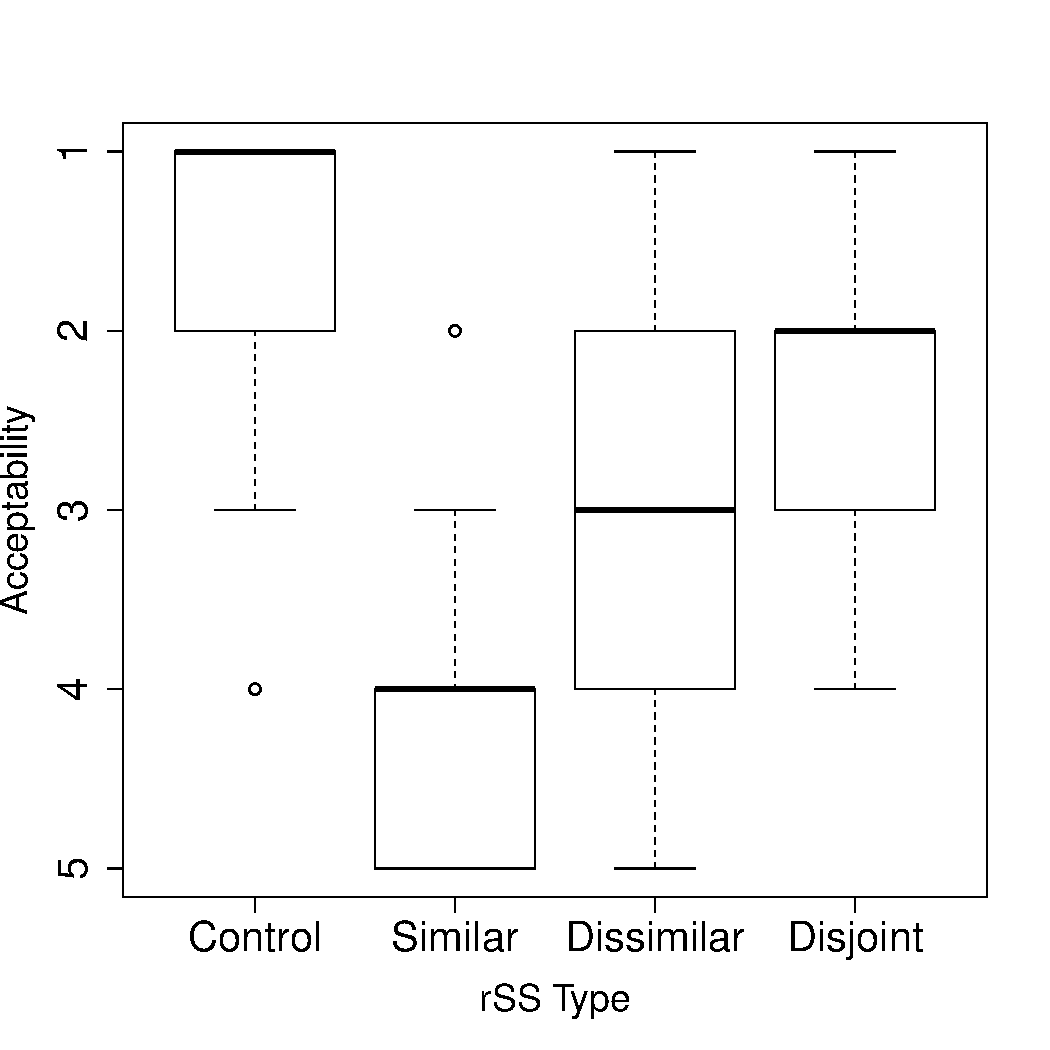
\includegraphics[page=1,width=0.425\linewidth]{boxplots.pdf}\hfill
\includegraphics[page=2,width=0.425\linewidth]{boxplots.pdf}
\end{minipage}
\caption{Boxplot for Cluster 1 (left) and Cluster 2 (right).}
\labfig{boxplot}
\end{figure}

One-tailed t-tests showed that, for Cluster 1, each condition is significantly different to every other condition. Comparing the {\scshape control} condition to the {\scshape disjoint} condition, we obtained $t(134)=-7.2, p<0.05$, to the {\scshape dissimilar} condition, $t(134)=-12.4, p<0.05$, and to the {\scshape similar} condition, $t(134)=-35.6, p<0.05$. Comparing the {\scshape similar} condition to the {\scshape dissimilar} condition, we obtain $t(134)=13.8, p<0.05$, and to the {\scshape disjoint} condition, $t(134)=23.6, p<0.05$. Comparing the {\scshape dissimilar} condition to the {\scshape disjoint} condition, we obtain $t(134)=6.4, p<0.05$.

For Cluster 2, the same one-tailed t-tests showed that each condition is significantly different to every other condition with the exception of the one-tailed t-test between {\scshape similarity} and {\scshape dissimilarity}, with $t(69)=-0.12, p>0.1$. Comparing the {\scshape control} condition to the {\scshape disjoint} condition, we obtained $t(69)=-5.1, p<0.05$, to the {\scshape dissimilar} condition, $t(69)=-23.6, p<0.05$, and to the {\scshape similar} condition, $t(69)=-27.7, p<0.05$. Comparing the {\scshape similar} to the {\scshape disjoint} condition, we obtained $t(69)=20.1, p<0.05$. Comparing the {\scshape dissimilar} condition to the {\scshape disjoint} condition, we obtain $t(69)=16.2, p<0.05$.


\subsection{Discussion}\labsec{discussion}
Our experiment set out to test two independent hypotheses, repeated below.
\begin{enumerate}
    \item If two reverse Sobel sequences are the same except for the degree of similarity between their conditionals' antecedent worlds, then the reverse Sobel sequence whose degree of similarity is more disparate should be considered more acceptable on average. (the \textit{dissimilar worlds hypothesis})
    \item If the domains of quantification of a reverse Sobel sequence are entirely disjoint, there should be no difference in acceptability between them and regular sentences (i.e. the control items). (the \textit{disjoint domain hypothesis})
\end{enumerate}
It is to be kept in mind that the second hypothesis mainly serves the purpose of establishing a positive baseline of acceptability for the results gathered from testing the first hypothesis.

\subsubsection{Disjoint Domain Hypothesis}\labsec{secondhypo}
Concerning the disjoint domain hypothesis, the results are quite clear: Since there is a significant difference between the {\scshape control} condition and the {\scshape disjoint} condition, and the latter is less acceptable on average, the null hypothesis has been falsified. However, the {\scshape disjoint} reverse Sobel sequences are, on average, only 0.67 points less acceptable than the control items. They are also far more acceptable than the other types of reverse Sobel sequences. We reckon that this slight---though significant---degradation in acceptability may be chalked up to the markedness of reverse Sobel sequences in general: The markedness of going from a specific case to a more general case that then seemingly contradicts the specific case, even if only on the surface. Generally speaking, in language, the reverse appears far more common (e.g. precisification). In the same line of reasoning, it appears, to us at least, quite difficult to find a natural occurrence of reverse Sobel sequences within any given corpus---written or spoken.

As such, we may consider the optimal reverse Sobel sequence acceptability to be below that of other, more typical utterances. The results of the dissimilar worlds hypothesis should therefore be contrasted against the results gathered from this hypothesis as a positive baseline, and not merely to the control items that consists of non-reverse Sobel sequences (amongst other utterance types).

\subsubsection{Dissimilar Worlds Hypothesis}\labsec{firsthypo}
For the dissimilar worlds hypothesis, the experiment yielded somewhat contradictory results. In \refsec{results}, it was shown that, for the undivided participant population, the {\scshape similar} condition is significantly different from the {\scshape dissimilar} condition and that the {\scshape dissimilar} condition yields higher values of acceptability than the {\scshape similar} condition by approximately one point of acceptability on average. As such, the hypothesis was technically confirmed, though the difference in acceptability was somewhat smaller and the variance of the {\scshape dissimilar} condition much higher than anticipated. However, the k-means cluster analysis has shown that there are actually two distinct population clusters within our group of participants. Cluster~1 continued to rate the {\scshape dissimilar} condition significantly higher in acceptability than the {\scshape similar} condition, now by approximately 1.5 points, but Cluster 2 appears to make no distinction between the two conditions whatsoever. Not only that, but the variance for the {\scshape dissimilar} condition in the first population cluster is still very high ($\sigma^2=1.21$) and the actual distribution of acceptability judgements disconcertingly even across the board, as seen in \reffig{boxplot}. As such, it seems that the participants in the first population cluster were unsure of what to do with these reverse Sobel sequence, rather than considering them a simple improvement on the {\scshape similar} condition's reverse Sobel sequence. Furthermore, both population clusters rate the {\scshape dissimilar} condition as less acceptable than the {\scshape disjoint} condition, meaning that even very dissimilar worlds do not automatically yield a reverse Sobel sequence whose acceptability rating could be considered as optimal.

These findings are unexpected by or contradictory to \citepos{Lewis2018} account, though to different degrees. If considered only on its own, Cluster 2 would directly falsify the dissimilar worlds hypothesis. The variance of Cluster 1 would suggest that dissimilarity---whilst clearly having a positive impact on acceptability in some cases---is not the sole deciding factor (aside from relevance) behind acceptability.

We must consider whether these two findings may be explained by \citepos{Lewis2018} model in its current state. Concerning Cluster 2, there are two explanations apparent to us: First, as the world closeness is an interaction between similarity and relevance, it might be the case that the participants of this population cluster consistently ascribe enough relevance to the $\phi\land\psi$-worlds s.t. they are always moved to be amongst the closest $\phi$-worlds irrespective of dissimilarity. The second possibility would be that they interpret the {\scshape dissimilar} $\phi\land\psi$-worlds as more similar than intended. The latter option would indicate that there might be an error in the experiment's design; more specifically, in how the {\scshape dissimilar} condition items were created. The former option would introduce the question why these participants would consistently go through the trouble of rearranging their world ordering -- even though most people would not, given the disparity in similarity -- if this leads to a contradictory reading. Both by principle of economy and charitability, it would be more suitable to leave the $\phi\land\psi$-worlds in their original place in the world ordering, given the vast distance they would have to cross to count amongst the closest $\phi$-worlds. Concerning the variance of the first population cluster, we have a similar option to argue in favour of \citepos{Lewis2018} model: If we were to assume that the $\phi\land\psi$-worlds of the {\scshape dissimilar} condition are regarded as more similar than intended, then the participants might be more inclined to provide them with lower acceptability ratings---the higher ratings would then be an act of charitable interpretation on their part. This would however raise the question why their charitability---a successful strategy---is only intermittently employed.

Excluding, for the sake of argument, the possibility of there being an inherent flaw in the design of the {\scshape dissimilar} reverse Sobel sequences and assuming that Cluster 2 is not that anti-charitable, we would argue that our results, whilst weakly supporting the dissimilar worlds hypothesis, are more contradictory to than supportive of \citepos{Lewis2018} model. Rather, the data would suggest to us that there is another main factor behind the acceptability of reverse Sobel sequence, as further explored in \refsec{introspection}.

\section{Felicity Factors for Reverse Sobel Sequences}\labsec{introspection}
In \refsec{firsthypo}, we argued that the experimental results suggest that relevance and dissimilarity may not be the only important factors for the acceptability of reverse Sobel sequences -- perhaps not even the main ones. What, then, renders reverse Sobel sequences acceptable in the rare instances when this is the case? From the results of the {\scshape disjoint} condition, we know that its ingredients are a recipe for (limited) success. Recalling the conditions for their creation from \refsec{materials}, we know them to be (i) establishing the $\phi\land\psi$-conditional as pertaining to epistemically excluded possibilities, whilst making the $\phi$-conditional a regular future-less-vivid conditional pertaining to live possibilities and (ii) having both sequence conditionals share a common discourse goal explicitly named by a sentence following the reverse Sobel sequence. As such, we tried to pin down what makes a reverse Sobel sequence acceptable by systematically creating reverse Sobel sequences with only one of these features or even neither of them whilst trying to keep the changes to a minimum. As we demonstrate on the following pages, native speaker acceptability judgements showed that (i) causal relations between the antecedent's propositions has the effect \textcite{Klecha2014} observed, (ii) reverse causal Sobel sequences are only felicitous if the relevance of $\phi\land\psi$ is denigrated or $\phi\land\psi$ is considered an epistemically excluded possibility, (iii) non-counterfactual reverse Sobel sequences are infelicitous unless the possibility of $\phi\land\psi$ is overtly denigrated, and that (iv) a unified discourse purpose is not required for felicity. 

First, we show that a unified discourse purpose is not required for felicity with the already existing example \refex{match}, repeated below as \refex{match-repeat3}:
\ex\phantomsection\context{Holding up a dry match, with no water around.}If I had struck this match and it had been soaked, it would not have lit. But if I \MakeUppercase{had} struck this match, it would have lit.\\%
\emptyfill(adapted from \textcite[p. 106]{Stalnaker1968} by \textcite[p. 487]{Lewis2018})\labex{match-repeat3}
\xe
Arguably, \refex{match-repeat3} is felicitous, even though there is no inherently clear discourse purpose shared by both conditionals. It could be argued that the shared purpose behind the sequence is to make the point that wet matches don't generally light when struck, but contexts are easily imaginable where the reverse Sobel sequence is merely uttered to reflect the reality of the match's dryness and what would have happened to it, if it had been struck. If this were to already count as a shared discourse purpose, it would be so broad in range that almost any non-incoherent discourse could be constructed as having a shared purpose in that sense, rendering it a non-factor anyhow.

Having excluded a shared discourse purpose as a relevant factor, we would posit the empirical breakdown in \reftab{ourdata}, where the corresponding example numbers that demonstrate this are given in brackets:%
\begin{table}[!htb]
\caption{Current empirical data on felicity distribution, broken down by causality, counterfactuality, and overt denigration of relevance (or implicit epistemic exclusion) of $\psi$, with example numbers that exemplify each reverse Sobel sequence condition. Contrastive stress on the auxiliary verb is assumed for all reverse Sobel sequences.}
\resizebox{\textwidth}{!}{
    \begin{tabular}{lcccccccc}\toprule
                &   \multicolumn{4}{c}{Acausal}     &  \multicolumn{4}{c}{Causal}\\
                & \multicolumn{2}{c}{Non-Counterfactual}  &   \multicolumn{2}{c}{Counterfactual}    & \multicolumn{2}{c}{Non-Counterfactual}  &   \multicolumn{2}{c}{Counterfactual}\\
                & Non-Denigrated & Denigrated  & Non-Denigrated & Denigrated   & Non-Denigrated & Denigrated & Non-Denigrated & Denigrated\\\midrule
          SS    &   \checkmark  & \checkmark &   \checkmark  &   \checkmark  &   \checkmark    &   \checkmark  &   \checkmark & \checkmark\\
          rSS   &   \#\refex{matchtomorrow}  & \checkmark\refex{acausalncfdenigrated}  & \checkmark\refex{match-repeat4}  &   \checkmark\refex{match-acausal-denigrated}  &   \#\refex{matchsnapnocf} & \checkmark\refex{causalncfdenigrated} &   \#\refex{matchsnapcf}    &   \checkmark\refex{match-causal-denigrated}\\
          \bottomrule
    \end{tabular}}\labtab{ourdata}
\end{table}

Crucially, it would appear that non-counterfactual and non-epistemically excluded possibility reverse Sobel sequences are typically infelicitous, as demonstrated with the reverse Sobel sequences in \refex{matchtomorrow} and \refex{matchsnapnocf}:
\ex\phantomsection\context{Concerning a dry match in a room with a large open source of water.}
    If I struck this match tomorrow and it was wet, it wouldn't light; \#but if I \MakeUppercase{were} to strike this match tomorrow, it would light.\labex{matchtomorrow}
\xe
\ex\phantomsection\context{Holding up a dry match (with no water around).}If I struck this match and it snapped, it would not light. \#But if I \MakeUppercase{were} to strike this match, it would light.\labex{matchsnapnocf}
\xe
This extends to all forms of non-counterfactual reverse Sobel sequences. As such, not only are future-less-vivid sequences infelicitous (as shown in \refex{matchtomorrow} and \refex{matchsnapnocf}), but their indicative counterparts as well, as shown in \refex{matchtomorrow-indicative} and \refex{matchsnapnocf-indicative}.
\ex\phantomsection\context{Concerning a dry match in a room with a large open source of water.}
    If I strike this match tomorrow and it is wet, it will not light; \#but if I \MakeUppercase{do} strike this match tomorrow, it will light.\labex{matchtomorrow-indicative}
\xe
\ex\phantomsection\context{Holding up a dry match (with no water around).}If I strike this match and it snaps, it will not light. \#But if I \MakeUppercase{do} strike this match, it will light.\labex{matchsnapnocf-indicative}
\xe

This may only be remedied by overtly questioning the relevance of $\phi\land\psi$ (or implicitly knowing of the quasi-impossibility and resulting irrelevance of $\psi$). If this is appropriately done, the reverse Sobel sequence is rendered felicitous, regardless of whether or not there is a causal relation between $\phi$ and $\psi$. This is demonstrated by \refex{acausalncfdenigrated}-\refex{causalncfdenigrated-indicative}.
\ex\phantomsection\context{Concerning a dry match in a room with a large open source of water.}
    If I struck this match tomorrow and it was wet, it wouldn't light. But there is little chance of this match becoming wet; so, if I \MakeUppercase{were} to strike this match tomorrow, it would light.\labex{acausalncfdenigrated}
\xe
\ex\phantomsection\context{Holding up a dry match (with no water around).}If I struck this match and it snapped, it would not light. But the chances of me snapping a match are really, really low; so, if I \MakeUppercase{were} to strike this match, it would light.\labex{causalncfdenigrated}
\xe
\ex\phantomsection\context{Concerning a dry match in a room with a large open source of water.}
    If I strike this match tomorrow and it is wet, it will not light. But there is little chance of this match becoming wet; so, if I \MakeUppercase{do} strike this match tomorrow, it will light.\labex{acausalncfdenigrated-indicative}
\xe
\ex\phantomsection\context{Holding up a dry match (with no water around).}If I strike this match and it snaps, it will not light. But the chances of me snapping a match are really, really low; so, if I \MakeUppercase{do} strike this match, it will light.\labex{causalncfdenigrated-indicative}
\xe

If a reverse Sobel sequence is counterfactual by nature, it would appear that they are always felicitous so long as $\phi$ and $\psi$ are causally unrelated (i.e., they are an acausal Sobel sequence), regardless of how dissimilar the worlds are to each other. This is demonstrated by \refex{match-repeat4} and \refex{match-similar}:
\ex\phantomsection\context{Holding up a dry match, with no water around.}If I had struck this match and it had been soaked, it would not have lit. But if I \MakeUppercase{had} struck this match, it would have lit.\\%
\emptyfill(adapted from \textcite[p. 106]{Stalnaker1968} by \textcite[p. 487]{Lewis2018})\labex{match-repeat4}
\xe
\ex\phantomsection\labex{match-similar}\context{Talking about a match that was dry but in a room with a large and open source of water; though the match did not get wet until being held by the speaker, it easily could have, had it moved even a little bit differently.}If I had struck this match and it had been soaked, it would not have lit. But if I \MakeUppercase{had} struck this match, it would have lit.
\xe

If there was some causal relation between $\phi$ and $\psi$, however, then, as \textcite{Klecha2014} already observed, the reverse Sobel sequence would be infelicitous, barring any intervention, as seen in \refex{matchsnapcf}:
\ex\phantomsection\context{Holding up a dry match (with no water around).}If I had struck this match and it had snapped, it would not have lit. \#But if I \MakeUppercase{had} struck this match, it would have lit.\labex{matchsnapcf}
\xe

Finally, causal and acausal reverse Sobel sequence may be rendered felicitous, if the relevance of $\phi\land\psi$ is appropriately denigrated via questioning its probability, as seen with the reverse Sobel sequences in \refex{match-acausal-denigrated} and \refex{match-causal-denigrated}:
\ex\phantomsection\context{Holding up a dry match, with no water around.}If I had struck this match and it had been soaked, it would not have lit. But, as we know, this match is dry, so if I \MakeUppercase{had} struck this match, it would have lit.\labex{match-acausal-denigrated}
\xe
\ex\phantomsection\context{Holding up a dry match (with no water around).}If I had struck this match and it had snapped, it wouldn't have lit. But the chances of the match breaking would've been very, very, \MakeUppercase{very} low, since I know what I'm doing. So, if I \MakeUppercase{had} struck this match, it would have lit.\labex{match-causal-denigrated}
\xe

With this, we may have identified the factor that threw off the results for the {\scshape similar} reverse Sobel sequences in \refsec{experiment}. In fact, considering the results from our experiment and that we have found no reverse Sobel sequences for which dissimilarity appears to play a role in felicity (short of the $\phi\land\psi$-worlds being so dissimilar that they ought to be considered excluded possibilities), we would argue that \citepos{Lewis2018} criterion of worlds having to be \enquote{similar enough} may be formally dropped: In the terminology of \textcite{Lewis2018}, any two sets of worlds appear similar enough so long as there is no counterfactuality or epistemically excluded possibility involved. Only if a reverse Sobel sequence involves a set of counterfactual or epistemically excluded worlds does similarity play a role in whether or not the sequence is rendered felicitous or infelicitous (in the sense of $\phi$ and $\phi\land\psi$ should not be equal in similarity). 

Having identified the criteria for reverse Sobel sequence felicity, we must now adopt some formal mechanism(s) whose predictions match the empirical data found within this chapter. We pursue this objective in \refch{pragmatics-SS}.
